\chapter{Marco teórico}
\label{chapter:marco:teorico}


\section{Programación paralela}

La programación paralela es una técnica de programación basada en la ejecución simultánea de instrucciones tanto en un mismo ordenador con varios procesadores o bien en un clúster conformado por varios ordenadores haciendo uso de la computación distribuida.
Los sistemas multiprocesadores consiguen un aumento del rendimiento si se utilizan estas técnicas. En los sistemas monoprocesador el beneficio en rendimiento no es tan evidente debido a que la CPU es compartida por múltiples procesos en el tiempo.
\newline El mayor problema de la computación paralela radica en la complejidad de la comunicación y sincronización de las tareas involucradas en la computación, ya sea mediante secciones críticas, semáforos o paso de mensajes que permitan garantizar la exclusión mutua en las zonas del código en las que sea necesario.
\newline El paradigma de diseño y programación difiere mucho del utilizado para diseñar y programar aplicaciones secuenciales. Aquí, una buena estrategia de división del problema puede determinar la eficiencia de un algoritmo paralelo.

\subsection{Computación paralela}

Se denomina computación paralela al procesamiento simultáneo de datos. Ésto se logra dividiendo el problema original en partes más pequeñas de manera tal que cada elemento de procesamiento pueda ejecutar una parte del algoritmo al mismo tiempo que los demás. \newline La idea principal de la computación paralela es poder ejecutar más instrucciones en menos tiempo, por más que las instrucciones sigan tardando lo mismo.
Los elementos de procesamiento pueden ser diversos e incluir recursos tales como un único ordenador con muchos procesadores, varios ordenadores en red, hardware especializado o una combinación de los anteriores.
Resumiendo, el objetivo primordial de la computación paralela es aumentar la velocidad computacional y reducir los tiempos en la resolución de problemas.

\textbf{\newline \large Tipos de paralelismo}

\textbf{\newline Paralelismo a nivel de bit:} se basa en el incremento del tamaño de la palabra\footnote{una palabra es una cadena finita de bits que son manejados como un conjunto por el procesador. El tamaño o longitud de una palabra hace referencia al número de bits contenidos en ella.} del procesador. 
 Incrementando el tamaño de la palabra se reduce el número de instrucciones que el procesador debe ejecutar al efectuar operaciones con variables cuyos tamaños son mayores a la longitud de su palabra. Por ejemplo, en el caso en que un procesador de 32 bits deba efectuar una suma de dos variables enteras de 64 bits, primero debe sumar los 32 bits más bajos de cada entero y luego sumar los 32 bits restantes, efectuando de esta manera un total de dos instrucciones para para resolver una única operación. En cambio, 
 si el procesador fuera de 64 bits esta operación se ejecutaría con una simple instrucción.

\textbf{\newline Paralelismo a nivel de instrucción:} es una técnica que busca combinar las instrucciones de bajo nivel ejecutadas por el procesador con el fin de encontrar el mejor orden de ejecución que permita correr instrucciones de manera simultánea sin afectar el resultado final. La idea principal de utilizar esta técnica es poder aumentar la velocidad de ejecución y aprovechar al máximo la capacidad del hardware.
 
\textbf{\newline Paralelismo a nivel de datos:} consiste en subdividir los datos de entrada de un programa y ejecutar en diferentes procesos la misma secuencia de operaciones sobre cada subconjunto obtenido en la división. Es decir, cada procesador ejecuta la misma tarea sobre diferentes conjuntos de datos. Aquí, los datos se distribuyen y las tareas se replican.

\textbf{\newline Paralelismo a nivel de tareas:} es un tipo de paralelización que se centra en la distribución de tareas a través de diferentes nodos de procesamiento. Lo que pretende este tipo de paralelismo es realizar una división del conjunto de tareas en subconjuntos más pequeños para que sean
 ejecutadas por los distintos nodos disponibles en la computación.
 A esta técnica también se la conoce como ``paralelismo funcional''.

\textbf{\newline \large Características principales}

\begin{itemize}
 \item Se utilizan múltiples núcleos de procesamiento para la ejecución de las tareas.
 \item Los problemas son divididos en partes más pequeñas o subproblemas de tal manera para que puedan ser resueltos en paralelo.
 \item Los subproblemas obtenidos de la división son ejecutados simultáneamente en núcleos diferentes.\\
\end{itemize}


\textbf{\newline \large Tipos de sistemas paralelos más conocidos} \vspace{5 mm} \\
Las computadoras paralelas pueden ser diferenciadas según el nivel en que su hardware soporta paralelismo. Existe una gran variedad de arquitecturas que permiten la ejecución simultánea de múltiples instrucciones:

\textbf{\newline Computación multi-núcleo:} está dada por un procesador conformado por múltiples núcleos de procesamiento en un mismo chip. Un procesador multi-núcleo puede ejecutar múltiples instrucciones por ciclo desde múltiples flujos de instrucciones.

\textbf{\newline Multi-procesamiento simétrico:} es un sistema informático con múltiples procesadores idénticos que comparten la memoria y se conectan mediante un bus.

\textbf{\newline Computación distribuida:} se utilizan varios ordenadores interconectados a quienes se les envían diferentes tareas para su computación. Cada ordenador ejecuta localmente ese trabajo y al finalizar lo reporta al ordenador central logrando de esta manera una ejecución paralela y distribuida de tareas. En la siguiente sección se darán más detalles al respecto.

\subsection{Taxonomía de Flynn}

La taxonomía de Flynn es una clasificación de arquitecturas de computadoras propuesta por Michael J. Flynn en 1966.\\
Las cuatro clasificaciones definidas por Flynn se basan en el número de instrucciones concurrentes y en los flujos de datos disponibles en la arquitectura.\\
\texttt{Flynn} creó cuatro clasificaciones distintas considerando si los programas y computadoras operaban sobre una o múltiples instrucciones y si esas instrucciones utilizan un solo conjunto o múltiples conjuntos de datos.\\

\textbf{\newline \large La Clasificación}

\textbf{\newline (SISD) Una instrucción, un dato:} del inglés ``Single Instruction Single Data'', es la computación secuencial que no explota el uso de paralelismo en las instrucciones ni tampoco en el flujo de datos. Un ejemplo de esta clasificación son las máquinas monoprocesador.\\

\textbf{\\Gráficamente:}
\begin{figure}[H]
\begin{center}
  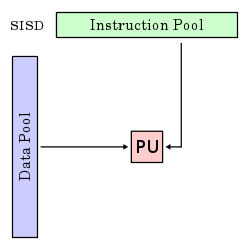
\includegraphics[scale=0.7]{images/SISD.png}
\caption{SISD}
\label{fig:SISD}
\end{center}
\end{figure} 

\textbf{\newline (SIMD) Una instrucción, múltiples datos:} del inglés ``Single Instruction Multiple Data'', es una arquitectura de computadora que explota múltiples flujos de datos en un único flujo de instrucciones para realizar operaciones las cuales pueden ser paralelizadas de manera natural. Por ejemplo: un GPU o un procesador vectorial el cual es capaz de ejecutar operaciones matemáticas sobre múltiples datos de forma simultánea.\\
\newpage

\textbf{\\Gráficamente: }

\begin{figure}[H]
\begin{center}
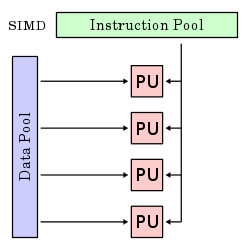
\includegraphics[scale=0.7]{images/SIMD.png}
\caption{SIMD}
\label{fig:SIMD}
\end{center}
\end{figure} 

\textbf{\newline (MISD) Múltiples instrucciones, un dato:} del inglés ``Multiple Instruction Single Data'', es una arquitectura que se utiliza cuando múltiples flujos de \linebreak instrucciones operan sobre un único flujo de datos. Esta arquitectura es poco común debido a que la efectividad de los múltiples flujos de instrucciones suele precisar de múltiples flujos de datos. Sistemas heterogéneos que operan sobre el mismo conjunto de datos y deben coincidir en resultados se suele utilizar en situaciones de paralelismo redundante, como por ejemplo en computadoras de control de navegación aérea, donde se necesitan varios sistemas de respaldo en caso de que uno falle.\\
\newpage 
\textbf{\\Gráficamente:}
\begin{figure}[H]
\begin{center}
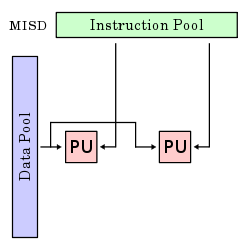
\includegraphics[scale=0.7]{images/MISD.png}
\caption{MISD}
\label{fig:MISD}
\end{center}
\end{figure} 

\textbf{\newline (MIMD) Múltiples instrucciones, múltiples datos:} del inglés ``Multiple Instruction Multiple Data'', esta arquitectura está conformada por múltiples procesadores autónomos que ejecutan simultáneamente diferentes instrucciones sobre conjuntos de datos diferentes. Los sistemas distribuidos por lo general son reconocidos en esta clasificación, ya sea explotando el uso de un único espacio compartido de memoria o bien uno distribuido.\\
\textbf{\\Gráficamente:}
\begin{figure}[H]
\begin{center}
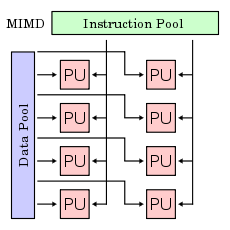
\includegraphics[scale=0.7]{images/MIMD.png}
\caption{MIMD}
\label{fig:MIMD}
\end{center}
\end{figure} 

El framework FuD presentado en la sección \ref{seccion:fud} tiene la capacidad de correr en máquinas con un diseño \textbf{MIMD}, con computadoras heterogéneas.


\subsection{Resolución de problemas paralelos}

El desarrollo de algoritmos paralelos aparece cuando tenemos un problema que requiere una gran capacidad de cómputo, ya sea por una gran cantidad de datos de entrada o por una gran complejidad en sus operaciones. El primer paso para el diseño de un algoritmo paralelo consiste en descomponer el problema principal en problemas más pequeños o subproblemas para que luego sean asignados a cada procesador y puedan ser ejecutados de manera independiente y simultánea.\\
No siempre es una buena decisión partir de un algoritmo secuencial intentando ``paralelizar'' la aplicación, sino que en ocasiones es necesario diseñar un nuevo algoritmo que seguramente será muy diferente al secuencial.

\textbf{\newline \large Descomposiciones más conocidas}

\textbf{\newline Descomposición de dominio o paralelismo de datos}: consiste en descomponer los datos de entrada de un programa 
paralelo en porciones más pequeñas e indivisibles de tal manera que posean aproximadamente el mismo tamaño. Cada una de estas porciones son asignadas a un procesador para su posterior ejecución. Se puede relacionar al paralelismo de datos con el modelo \textbf{SIMD} ya que permite mantener un único flujo de instrucciones.

\textbf{\newline Descomposición funcional}: se basa en la división del programa principal en subtareas más pequeñas donde cada una de éstas son asignadas y ejecutadas de manera independiente por cada procesador. En muchos casos, el número de subtareas obtenidas puede ser mayor a la cantidad de procesadores con los que se cuenta. \\
Este tipo de descomposición se implementa siguiendo un paradigma maestro-esclavo donde existe un proceso maestro que se encarga de enviar subtareas a los procesos
 esclavos. Cuando uno de estos últimos termina su computación, los resultados se envían al proceso maestro el cual nuevamente le asigna una nueva subtarea a procesar.
 Se prosigue de esta manera hasta agotar las subtareas pendientes.

\subsection{Modelos de programación paralela}

Los modelos de programación no están totalmente ligados a las arquitecturas paralelas pero sí estrechamente relacionados. Podríamos decir que cada arquitectura de computación paralela justifica esta relación haciendo uso de dichos modelos. Es por eso que un determinado modelos puede ser más eficiente que otro cuando se aplica sobre determinadas arquitecturas paralelas.\\
Existen básicamente dos modelos de comunicación de las plataformas paralelas \cite{gramagrubta}:

\textbf{\newline Espacios de direcciones compartidas \textit{(Shared Address Space)}}: se ve a los programas como una colección de procesos que pueden acceder a variables locales y globales almacenadas en un espacio de memoria compartido entre las diversas unidades de procesamiento. Cada proceso accede a dicha memoria a través de lecturas asincrónicas.\\
Este modelo es apropiado para el desarrollo de aplicaciones sobre arquitecturas de memoria compartida, aunque también puede ser utilizado para el desarrollo de aplicaciones sobre arquitecturas distribuidas, simulando un espacio de memoria compartido.

\textbf{\newline Paso de mensajes \textit{(Message Passing)}}: es una técnica empleada para aportar sincronización entre procesos y permitir la exclusión mutua de manera similar a como se hace con los semáforos, monitores, etc. Su principal característica es que no precisa de memoria compartida, por lo que es muy importante en la programación de sistemas distribuidos. Los elementos principales que intervienen en el paso de mensajes son: el proceso que envía, el que recibe y el mensaje.

\subsection{Equilibrio de carga}

Un aspecto fundamental que hay que tener en cuenta a la hora de desarrollar un programa paralelo es el \texttt{equilibrio de carga}.

Ésta es una metodología para distribuir equitativamente los trabajos a través de múltiples computadoras, clústers, procesos, redes de trabajos, discos, o todo aquello que conforme el sistema paralelo utilizado, de tal manera que se pueda asegurar el uso y la óptima distribución de los recursos para poder maximizar la salida, minimizar el tiempo de respuesta y evitar la sobrecarga en ciertos procesos cuando los demás se encuentren ociosos.

El equilibrio de carga se utiliza comúnmente para realizar comunicaciones internas en clústers o para implementar algoritmos de planificación en sistemas operativos.

\subsection{Etapas de diseño}

Las etapas de diseño de aplicaciones paralelas podrían resumirse entonces como sigue:
\begin{itemize}
 \item Identificar el trabajo que puede realizarse en paralelo.
 \item Diseñar la división y unificación del trabajo y datos entre procesos involucrados.
 \item Determinar el acceso a los datos, sincronizaciones y dependencias entre tareas.
 \item Asignar recursos de cómputo a los procesos que se ejecutarán en paralelo.
\end{itemize}


\section{Programación distribuida}

Un sistema distribuido se define como una colección de ordenadores autónomos conectados por una red y controlados por el software distribuido adecuado para que el sistema sea visto por los usuarios como una única entidad capaz de proporcionar facilidades de computación. El desarrollo de los sistemas distribuidos vino de la mano de las redes locales de alta velocidad
 a principios de \textit{1970}. Actualmente, la disponibilidad de computadoras personales de altas prestaciones, estaciones de trabajo y ordenadores servidores ha resultado en un mayor desplazamiento
 hacia los sistemas distribuidos respecto de los ordenadores centralizados multiusuario. Esta tendencia se ha acelerado por el desarrollo de software para sistemas distribuidos diseñado
 para soportar el desarrollo de aplicaciones distribuidas para permitir a los ordenadores coordinar sus actividades y compartir los recursos del sistema, hardware, software y datos.
Los sistemas distribuidos se implementan para hacer uso de diversas plataformas de hardware, desde unas pocas estaciones de trabajo conectadas por una red de área local, hasta Internet,
 que comunica a millones de ordenadores donde sus aplicaciones varían desde la provisión de capacidad de cómputo a grupos de usuarios, hasta sistemas bancarios, comunicaciones multimedia y
 abarcan prácticamente todas las aplicaciones comerciales y técnicas actuales. 

La programación distribuida es un tipo de programación paralela. Los programas paralelos pueden correr localmente y de manera coordinada, o bien estar separados en diferentes unidades de cómputo.
 Generalmente, en este último caso, los ordenadores suelen ser muy diferentes entre sí por lo que desarrollar este tipo de aplicaciones resulta en un mayor esfuerzo debido a nuevos factores que se
 deben tener en cuenta para mantener la calidad del software, como son la seguridad, extensibilidad, escalabilidad, tratamiento de fallos, concurrencia, transparencia del usuario frente a los componentes
 del sistema y heterogeneidad de los componentes  entre otros. Cuando se pretende resolver un problema de manera distribuida, el programa necesita ser dividido y cada parte resultante debe poder correr
 en diferentes ordenadores. Estos sub-programas corren simultáneamente y necesitan mantener una cierta comunicación entre sí que les permita avanzar con su respectiva tarea. 
Otro punto a tener en cuenta a la hora de desarrollar una aplicación distribuida es que si las aplicaciones van a correr en arquitecturas de hardware diferentes, 
estos programas tienen que ser compilados y optimizados específicamente para cada una.

\begin{center}
\begin{itshape}
 \textit{Programar un sistema distribuido significa escribir un programa para cada proceso tal que todos los programas en conjunto implementan la aplicación deseada \cite{VanRoyHaridi} }
\end{itshape}
\end{center}

La coordinación de estos procesos distribuidos puede ser una tarea complicada debido a que algunas unidades de trabajo pueden fallar o ser interrumpidas, o bien, los mensajes que contienen
 datos de entrada y/o resultados de la computación, podrían también no llegar a destino. Por consiguiente, si los programas se escriben sin contemplar estos casos, es probable que ante alguna
 situación de éstas, todas las computadoras involucradas en la resolución del problema terminen fracasando. En la programación distribuida, un proceso podría ser el proceso de control encargado 
de recibir y administrar los trabajos hechos por otros procesos, como es el caso de una arquitectura cliente-servidor donde el servidor debe manejar los requisitos de los clientes, o bien,
 todos los procesos podrían trabajar de manera peer-to-peer sin que exista un proceso maestro de control. Algunos ejemplos de problemas en donde se utiliza la programación distribuida para
 su resolución son, el análisis de datos geológicos sobre recursos como el petróleo, el modelado de proteínas y moléculas biológicas, la decodificación de mensajes, y simulaciones militares, entre otros.
 El proyecto \textsc{SETI} \footnote{\url{http://www.seti.org/}} encargado de buscar inteligencia extraterrestre utilizando ondas de radiofrecuencia capturadas desde la tierra quizás es uno de los mejores ejemplos.

Los sistemas distribuidos abarcan una cantidad de aspectos considerables, por lo cual su desarrollo implica mucha complejidad. En este modelo es muy importante que en las etapas de diseño y
 desarrollo se consideren dónde va a correr el sistema y cómo va a ser utilizado. Para ello, es necesario identificar ciertos puntos que son claves a la hora de diseñar y desarrollar una aplicación distribuida.
 Se debe identificar:

\begin{itemize}

 \item el tipo de Sistema Operativo sobre el cual correrá cada proceso,
 \item la red de comunicación que será utilizada,
 \item el lenguaje de programación que mejor se adapte a la solución del problema,
 \item qué debe hacer el servidor y qué debe hacer cada cliente,
 \item cómo actuar frente a pérdidas de mensajes, saturación en el tráfico, mensajes repetidos, 
 \item cómo mantener segura las conexiones,
 \item qué cantidad de clientes podrá manipular cada servidor,
 \item cómo descomponer el problema y cómo distribuir el trabajo de manera eficiente.

\end{itemize}
Estos puntos varían con cada problema sobre todo considerando los diferentes criterios e interpretaciones con los cuales puedan ser abordados.

Es importante que todas las aplicaciones incluyan un alto nivel de fiabilidad, seguridad contra interferencias externas y que proporcionen privacidad de toda la información que manejen.\\
 
\textbf{\newline Características de las aplicaciones distribuidas}\\
\\Concurrencia: los recursos disponibles en la red puedan ser utilizados simultáneamente por los usuarios y/o agentes que interactúan en la red. Por ejemplo el acceso simultáneo a la base de datos de un servidor.\\
\\Carencia de reloj global: las coordinaciones para la transferencia de mensajes entre los diferentes componentes para la realización de una tarea, no tienen una temporización general, está más bien distribuida a los componentes.\\
\\Fallos independientes de los componentes: cada componente del sistema puede fallar independientemente, con lo cual los demás pueden continuar ejecutando sus acciones.
 Esto permite el logro de las tareas con mayor efectividad, pues el sistema en su conjunto continúa trabajando.

\subsection{Topología de los sistemas distribuidos}

La topología de red se define como la cadena de comunicación usada por los nodos que conforman una red para comunicarse. 
En sistemas distribuidos, el término ``topología'' puede ser considerado y analizado en diversos contextos: físico, lógico o en términos de la comunicación, entre otros. Un caso particular es considerar la topología bajo el contexto del flujo de información. \\
Las topologías más comunes en este contexto son:

\begin{itemize}

 \item \textbf{Centralizada o Estrella}:

La topología estrella es uno de los tipos de topologías más utilizado donde generalmente las aplicaciones son vistas bajo una arquitectura cliente-servidor usado por servidores web, bases de datos y una amplia cantidad de sistemas distribuidos. Aquí, múltiples clientes se conectan a un único servidor quien es el encargado de centralizar y manejar toda la información disponible y de atender los requerimientos de los clientes. Por ejemplo, el proyecto \textsc{SETI@Home} es una arquitectura totalmente centralizada donde el servidor es el encargado de generar trabajos que luego serán computados por sus clientes. Entre sus ventajas se pueden mencionar: 

\begin{itemize}
\item si una PC se desconecta, o la conexión se pierde, solo queda fuera de la red esa PC,
\item resulta sencillo agregar y reconfigurar un nuevo ordenador,
\item es fácil prevenir daños o conflictos.
\end{itemize}

Una desventaja importante de esta topología es que si el nodo central falla, toda la red deja de transmitir.\\

\textbf{Gráficamente: }

\begin{figure}[H]
\begin{center}
  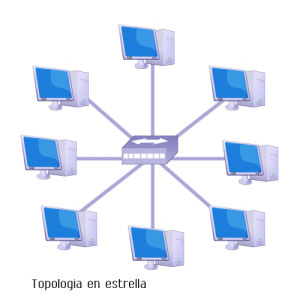
\includegraphics[height=2.5in,width=2.5in]{images/star.png}
\caption{Topología-estrella }
\label{fig:Estrella}
\end{center}
\end{figure} 

 \item \textbf{Anillo}:

En ocasiones, un único servidor centralizado no es capaz de manejar altas cargas de clientes, por lo que una solución común es utilizar un conjunto de ordenadores conectados en forma
 de anillo actuando como un único servidor distribuido. Aquí, cada estación está conectada a la siguiente y la última está conectada a la primera.
 Cada estación, además, tiene un receptor y un transmisor que hace la función de repetidor pasando la señal a la siguiente estación. En este tipo de red la comunicación
 se da por el paso de un token encargado de distribuir paquetes de información evitando de esta manera eventuales pérdidas de información debidas a colisiones.\\

\textbf{Gráficamente: }

\begin{figure}[H]
\begin{center}
  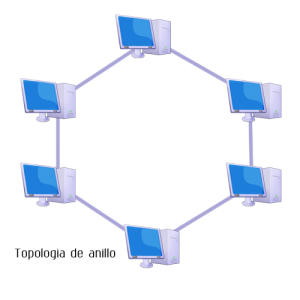
\includegraphics[height=2.5in,width=2.5in]{images/ring.png}
\caption{Topología-anillo }
\label{fig:Anillo}
\end{center}
\end{figure} 

 \item \textbf{Jerárquica o Árbol}

La topología jerárquica, también conocida como topología de árbol, tiene una larga historia en internet. Aquí  se cuenta con nodos periféricos individuales, por ejemplo hojas, que requieren transmitir  y recibir  únicamente de otros nodos sin la necesidad de actuar como repetidores o regeneradores. Al contrario de las redes centralizadas, la función del nodo central se puede distribuir. Como en las redes centralizadas convencionales, los nodos individuales pueden quedar aislados de la red por un fallo puntual en la ruta de conexión del nodo.
En estos casos, si falla un enlace que conecta con un nodo hoja, ese nodo hoja queda aislado; si falla un enlace con un nodo que no sea hoja, la sección entera queda aislada del resto.

Un ejemplo de este tipo de topología es la inserción del servicio de internet desde el proveedor, pasando por el router, luego por un switch que puede derivar a otro switch u otro router o sencillamente a los hosts. El resultado final, es una red con apariencia de árbol porque desde el primer router se comienza a ramificar la distribución de internet dando lugar a la creación de nuevas redes o subredes tanto internas como externas.

El sistema jerárquico más conocido en internet es el Servicio de Nombres de Dominio, \texttt{DNS}.\\
\newpage

\textbf{Gráficamente: }

\begin{figure}[H]
\begin{center}
  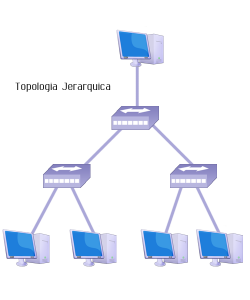
\includegraphics[height=2.5in,width=2.5in]{images/arbol.png}
\caption{Topología-arbol }
\label{fig:Arbol}
\end{center}
\end{figure} 

\item \textbf{Descentralizada}

Aquí, todos los nodos se comunican de manera simétrica y todos tienen las mismas funciones. Un ejemplo de este tipo de topología son las redes P2P, de las cuales Gnutella probablemente es el sistema puro descentralizado más conocido utilizado hoy en día. En las redes de este tipo, los nodos actúan como cliente y como servidor sin la necesidad de un servidor central que maneje las conexiones de red ni de un enrutador central que sirva como nodo y que administre direcciones. A esta topología también suele llamársela ``topología en malla''.
\newpage
\textbf{Gráficamente: }

\begin{figure}[H]
\begin{center}
  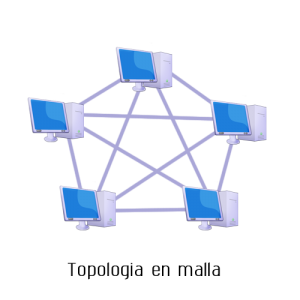
\includegraphics[height=2.5in,width=2.5in]{images/mesh.png}
\caption{Topología-decentralizada}
\label{fig:Decentralizado}
\end{center}
\end{figure} 

\item \textbf{Topologías Híbridas}

Las redes híbridas usan una combinación de dos o más topologías distintas de manera tal que la red resultante no tiene forma estándar. 
Por ejemplo, una red en árbol conectada a una red en árbol sigue siendo una red en árbol, pero dos redes en estrella conectadas entre sí  
muestran una topología de red híbrida. Estos tipos de redes se generan cuando se conectan dos topologías de red básicas. 

\textbf{Gráficamente: }

\begin{figure}[H]
\begin{center}
  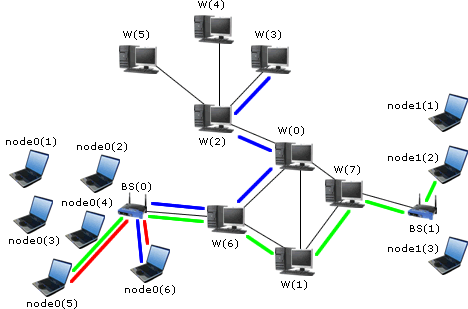
\includegraphics[height=2.5in,width=4.0in]{images/hibrida.png}
\caption{Topología híbrida}
\label{fig:Hibrida}
\end{center}
\end{figure} 

\end{itemize}

\subsection{Arquitectura cliente-servidor}

La arquitectura cliente-servidor de un sistema distribuido es el modelo más conocido y ampliamente adoptado en la actualidad. Consiste de una o varias aplicaciones servidoras,
 cada una actuando como un gestor de recursos y de una colección de aplicaciones clientes las cuales llevan a cabo tareas que requieren acceso a los recursos de hardware y/o software compartidos.
Los gestores de recursos a su vez podrían necesitar acceder a recursos compartidos manejados por otros procesos, es por eso que algunos procesos tienen ambos roles: son clientes y servidores a la vez. 

En este modelo, todos los recursos compartidos son mantenidos y manejados por los procesos servidores. Los procesos clientes realizan peticiones a los servidores cuando necesitan acceder a algún recurso.
Si la petición es válida, entonces el servidor lleva a cabo la acción requerida y envía una respuesta al proceso cliente.\\

Los servicios brindados varían de un sistema a otro, entre ellos se encuentran los siguientes:

\begin{itemize}
 \item  Ejecución de un determinado programa.
 \item  Acceso a un determinado banco de información.
 \item  Acceso a un dispositivo de hardware.
\end{itemize}

Esta arquitectura permite descentralizar el procesamiento y los recursos haciendo que ciertos servidores estén dedicados solo a una aplicación determinada y por lo tanto ejecutarla de manera eficiente.
Existen diversos tipos de servidores, entre los más comunes se encuentran los servidores de archivos, servidores de bases de datos, servidores web, servidores de correo, servidores de objetos, servidores de impresión, etc.


\section{Computación grid}

La computación Grid no es una nueva tecnología pero sí innovadora ya que representa una forma diferente de computación distribuida. Fue propuesta por Lan Foster y Carl Kesselman a mediados de los '90 como una revolucionaria técnica para resolver problemas complejos entre diversas organizaciones optimizando costos y tiempos. A partir del año 2000 se han hecho grandes progresos sobre dicha infraestructura y actualmente es cada vez más utilizada por organizaciones de todo el mundo.

Computación Grid puede tener varios significados para diferentes personas. La visión más general es presentada como una analogía a las redes de energía donde los usuarios tienen acceso a la electricidad a través de los enchufes de la pared sin importar ni considerar cómo y dónde se genera dicha energía. Esta visión presenta una idea donde la computación Grid se vuelve penetrante y los usuarios ganan acceso a recursos como les sea necesario sin tener conocimiento alguno sobre dónde se ubican dichos recursos o qué tipo de hardware y/o software poseen.

El término “Computación Grid” o simplemente “Grid” se enmarca dentro de la tecnología que permite agrupar un conjunto de recursos computacionales para resolver problemas de gran escala mediante el uso colectivo de ordenadores de escritorio, PDA, portátiles, móviles, redes, software, bases de datos, o instrumentos especiales como radios y telescopios. Es por ello que el propósito del grid es facilitar la correcta integración de todos estos recursos como un todo.
El control y mantenimiento central del Grid es llevado a cabo por un servidor que, generalmente, se encuentra replicado. Él es quien se ocupa de manejar y monitorizar el tráfico del sistema Grid encargándose de la entrega de los trabajos listos para procesar, de la recepción de resultados parciales y de la combinación de todos los resultados parciales para obtener el resultado final.

Puesto que los recursos que son compartidos pertenecen a diferentes usuarios, la seguridad pasa a ser un factor esencial en esta arquitectura centrándose en los siguientes aspectos:

\begin{itemize}
 \item \textbf{política de accesos:} define qué es lo que se va a compartir, a quién se le permite el acceso y bajo qué condiciones.
 \item \textbf{autenticación:} mecanismos para garantizar la identidad de un usuario o de un recurso concreto.
 \item \textbf{autorización:} procedimiento para averiguar si una determinada operación es consistente en base a las relaciones que se han definido previamente de cara a compartir recursos.
\end{itemize}

\textbf{Existen tres conceptos importantes que describen un Grid:}

\begin{itemize}
\item \textbf{visualización:} se refiere a la integración uniforme de sistemas heterogéneos geográficamente distribuidos que permiten a los usuarios hacer uso del Grid de manera transparente. Los nodos que conforman el Grid no están centrados geográficamente en un punto 	particular sino que están distribuidos en múltiples dominios y pueden ser accedidos a través de redes de área extensa, como por ejemplo Internet. Esta distribución implica que un usuario del Grid puede tener acceso directo a dichos nodos sin importar su ubicación pudiendo de esta manera extraer los recursos que requiera para el cómputo. Por ello, desde la perspectiva del usuario, hay un solo punto de entrada al sistema Grid.
\item \textbf{heterogeneidad:} representa la heterogeneidad de los recursos que forman las organizaciones virtuales que conforman al Grid. Es decir, que dichas organizaciones están compuestas por nodos de procesamiento que poseen hardware, software y sistemas operativos diferentes.
\item \textbf{dinámico:} los recursos pueden unirse o abandonar una organización virtual según conveniencia.
\end{itemize}

La principal utilidad del Grid es proveer de manera eficiente altas prestaciones de procesamiento con el fin reducir los tiempos en la resolución de problemas que requieren una gran capacidad de cómputo.

\begin{center}
\textit{“Grid es un súper-ordenador virtual que permite ejecutar aplicaciones que no pueden ser soportadas eficientemente en un único ordenador”}
\end{center}

\textbf{Clasificación de la Computación Grid:}

Podemos encontrar diversos tipos de Computación Grid. Éstos se clasifican según los servicios y recursos que ofrecen a los usuarios:

\begin{itemize}

\item \textbf{Grid Computacionales:} permite el acceso a los llamados “súper-computadores” para realizar tareas que requieren tiempos de cálculos muy elevados.
  
\item \textbf{Grid específicos:} en esta clasificación se engloban los Grids utilizados para ciertas investigaciones sobre temas específicos. 
Algunos de los temas para los que se utilizan son farmacéutica, química, astrofísica, tratamiento y representación de videos, simulación del clima, geología, etc.

\item \textbf{Grid de datos:} orientado principalmente para un almacenamiento y replicado de datos desde sitios ubicados en distintos sectores geográficos. Su funcionalidad se centra en obtención, catalogación, replicación y la coordinación de grandes cantidades de datos.

\item \textbf{Grid de servicios:} su funcionalidad se centra en proporcionar a los clientes recursos y aplicaciones desde cualquier componente de 
la arquitectura Grid a través de alguna política de disponibilidad (autoría, reconocimiento, etc.).

\item \textbf{Grid de recursos:} a diferencia del anterior, su funcionalidad se centra en proveer a los usuarios el uso de recursos concretos tales como capacidad de cómputo, ciclos de CPU, etc. desde un sector o área específica de la arquitectura grid.

\end{itemize}

\vspace{0,5cm}

\textbf{Características de la computación Grid:}

\begin{itemize}
\item \textbf{capacidad de equilibrio de sistemas:} los usuarios no necesitan calcular la capacidad de cómputo de los ordenadores a la hora de la entrega de trabajos ya que si ese ordenador no posee los recursos suficientes para llevarlo a cabo, el middleware reasignará el trabajo a otro ordenador.
\item \textbf{bajo costo:} brinda el poder de un súper-computador a un bajo costo ya que se dispone de una ``Grilla'' de recursos. No es necesario disponer de grandes servidores sino que se hace uso de componentes de bajo costo como lo son las PC de escritorio, laptops, etc.
\item \textbf{alta disponibilidad:} Si uno de los servidores falla, se reasignarán sus servicios a los servidores restantes.
\item \textbf{tolerancia a fallos:} si uno de los nodos del Grid falla, el sistema lo reconoce y reasignará la tarea a otra máquina. 
\item es una estructura flexible a los cambios.
\item no necesita de nuevas estructuras o arquitecturas para que funcione.
\end{itemize}

\vspace{0,5cm}

\textbf{Proyectos más conocidos que hacen uso de la Computación Grid:}

\begin{itemize}
  
\item SETI@Home \url{http://setiathome.berkeley.edu/}
\item Folding@Home \url{http://folding.stanford.edu/Spanish/Main/}
\item EGEE \url{http://public.eu-egee.org/}
\item IrisGrid \url{http://www.irisgrid.es/}
\item EELA \url{ http://www.eu-eela.org/}
\item EUFORIA \url{http://www.euforia-project.eu/}

\end{itemize}

\vspace{0,5cm}

\textbf{ Herramientas para implementar proyectos Grid:}

\begin{itemize}
 \item  BOINC \url{http://boinc.berkeley.edu/}
 \item  Advance Resource Connector \url{http://www.nordugrid.org/middleware/}
 \item  Load Sharing Facility \url{http://www.platform.com/Products/platform-lsf-family/}
 \item  Parallel Virtual Machine \url{http://www.csm.ornl.gov/pvm/pvm_home.html}
 \item  Globus Toolkit \url{http://www.globus.org/}
\end{itemize}

\textbf{Características de los servicios ofrecidos por la infraestructura del grid:}

\begin{itemize}
\item Servicios seguros en cuanto a capacidad de cómputo, integridad de datos, acceso a recursos, etc.
\item Servicio consistente basado en estándares evitando la heterogeneidad en el acceso a datos y operaciones.
\item Servicio penetrante ya que desde cualquier ubicación se puede acceder a sus recursos y extraer la potencia que se requiera.
\item Servicio económico lo que permite que llegue a más organizaciones haciendo que esta tecnología se universalice.
\end{itemize}


\subsection{Arquitectura de un sistema Grid}

Para lograr conseguir una imagen comprensible y coherente de la arquitectura de un sistema Grid es necesario primeramente identificar aquellos 
servicios que son necesarios en todo sistema y que, precisamente, son los que brindan las propiedades y características más destacadas.  

\subsubsection{ Servicios requeridos }

Para hacer posible que la ejecución de un trabajo sea satisfactoria se requieren de unos servicios que provean la funcionalidad que este trabajo requiera: 

\begin{itemize}

\item Por ejemplo, un usuario debe poder identificarse. Con este servicio el usuario puede certificar que es realmente quien dice ser, y
 asimismo el recurso que se quiere utilizar deberá autenticarse para que el usuario tenga la seguridad de que se ejecuta donde quiere, por lo que hablamos de autenticación mutua.
\item Un servicio de autorización es necesario, también para permitirle a un usuario la ejecución de tareas sobre un recurso, autorizándose como un usuario local, 
con sus permisos y restricciones dependiendo del contexto, la hora de petición o ejecución, etcétera.
\item Un servicio de planificación o  scheduling de los recursos, para que la utilización de los mismos sea eficiente y haya un reparto equitativo.
\item Asimismo es necesario un servicio para  descubrir recursos, ya que en un entorno de estas características se pueden añadir y quitar los mismos por
 lo que su selección debe ser dinámica.
\item También es recomendable un servicio de reserva anticipada, para poder ejecutar en un grupo de recursos en los que normalmente no es posible hacerlo,
 y que debe compenetrarse con el servicio de planificación.
\item Un servicio de  acceso a datos remotos, necesario para obtener los datos requeridos por un programa en ejecución ya que éstos pueden ser muy numerosos.
 Puede ser necesario un servicio de  réplica  para hacer copias de datos que sean muy “caros” de  transportar y que pueda ser conveniente tener en una localización más cercana.
\item Además se debe contar con recursos para hacer transferencias rápidas de estos datos.
\item Los servicios de  monitorización  son necesarios para controlar la correcta ejecución de los distintos trabajos, así como para controlar si los diferentes 
servicios que hemos comentado se encuentran disponibles y corriendo correctamente para su utilización.

\end{itemize}

\subsubsection{Arquitectura global}

La arquitectura global del sistema puede dividirse en diferentes piezas, dependiendo de los diferentes niveles en los que actúe cada componente. Ésto nos dará un típico modelo de arquitectura en capas.

\begin{figure}[H]
\begin{center}
  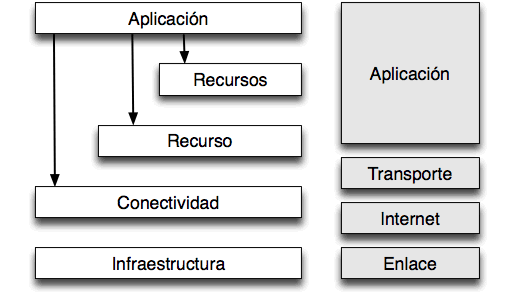
\includegraphics[height=3.0in,width=4.0in]{images/arquitectura-grid.png}
\caption{Arquitectura-Global}
\label{fig:Arquitectura}
\end{center}
\end{figure}

\begin{itemize}
 \item  En el nivel más bajo encontramos los servicios que son aplicables al control de los recursos locales, es lo que se denomina la capa \textbf{fábrica} o \textbf{infraestructura}.
 En esta capa se modelan los recursos accesibles, aquellos como:

      \begin{itemize}
      \item Recursos computacionales, como por ejemplo un clúster o un simple computador personal.
      \item Sensores, instrumentos de laboratorio.
      \item Sistemas de almacenamiento de datos.
      \item Sistemas de archivos distribuidos.
      \end{itemize}

      La funcionalidad básica que deben proveer, y de la que dependen capas superiores es la que nos da información sobre los recursos que está 
      modelando y de qué manera están disponibles para su utilización. Por ejemplo, para recursos computacionales debe:

      \begin{itemize}
      \item proveer información sobre el Hardware y el Software disponible, sobre el estado actual, carga, utilización, disponibilidad etcétera.
      \item monitorizar procesos que se estén ejecutando.
      \item un valor opcional podría ser la posibilidad de reservar el recurso.
      \item controlar recursos asociados a procesos.
      \item dar información sobre el estado de una posible cola de ejecución en la que residan los procesos.
      \end{itemize}

\item  En el siguiente nivel, nos encontramos con la capa de \textbf{Conectividad}, que tiene como función proveer los métodos y protocolos de comunicación entre los 
recursos modelados en la capa anterior. Aquí, los protocolos y la seguridad son muy importantes ya que es un requerimiento básico para el correcto funcionamiento del sistema. 
En esta capa se encuentran servicios que proveen los medios adecuados para hacer posible la comunicación a cualquier middleware o aplicación que se encuentre por encima de estos.

\item La siguiente capa es la denominada de \textbf{Recurso}, y es la encargada de compartir y gestionar los recursos individuales mediante la utilización de protocolos sobre la capa anterior de conectividad. En esta capa se definen los protocolos que permiten monitorizar, controlar y negociar operaciones que requieren un único recurso mediante los servicios subyacentes. 
Además, se llevarán a cabo la iniciación de las transacciones que sean necesarias para la realización del trabajo, tales como la comunicación 
del ejecutable en el recurso en el que se vaya a ejecutar, así también como la localización y recuperación de aquellos datos que sean necesarios para la ejecución.
También debe ser posible realizar en esta capa el control de los trabajos, proporcionando los métodos para reiniciar, relocalizar o cancelar un trabajo. 
Dentro de este control también podemos incluir en parte los servicios de Accounting, quienes permiten llevar un registro estadístico de las aplicaciones que 
se han corrido en un determinado recurso.

\item  La siguiente capa es la denominada capa de \textbf{Recursos}, y tiene como finalidad la coordinación de múltiples recursos accesibles por la capa anterior. En esta capa podemos encontrar, por ejemplo, aquellos servicios de información y directorio que nos dan una idea global del sistema y  mediante los cuales podemos localizar los recursos necesarios. La función principal aquí es la de utilizar los protocolos de comunicación de información de la capa anterior para proveer una vista global de los recursos. Aquí se sitúan servicios como los de \textit{scheduling}, \textit{co-allocation}, y \textit{brokering}. Estos servicios proveen los métodos para buscar aquellos recursos que se adaptan a las necesidades de nuestros trabajos, conociendo algunos datos sobre los mismos e intentando optimizar la asignación global mediante métodos de búsqueda o brokering. Con los servicios de \textit{co-allocation} podemos hacer reservas simultáneas de aquellos recursos que son necesarios para la consecución correcta del trabajo.

      \textbf{Existen tres tipos distintos de scheduler distribuido:}
      \begin{itemize}
      \item  Planificador de trabajos, encargado de maximizar los trabajos realizados por unidad de tiempo.
      \item  Planificador de recursos, encargado de llevar al máximo posible el uso de los recursos disponibles.
      \item  Planificador de la aplicación, encargado de dividir la aplicación en tareas, asignar los recursos necesarios para su ejecución y monitorizar el desarrollo de los mismos.
      \end{itemize}

      Los dos primeros intentan asegurar la eficiencia del grid, mientras que el tercero se enfoca exclusivamente en la efectividad de la aplicación.\\

      Esta capa también puede incluir servicios de replicación de datos, por ejemplo en caso de que estuvieran en una localización lejana.
      Las capas más altas como las aplicaciones o servicios más complejos del middleware deben utilizar los servicios que se provean en esta capa para la programación del grid. 

\item La siguiente y última capa es la denominada de \textbf{aplicación}, la cual se enfoca a la definición de protocolos que permitan a las aplicaciones acceder al grid a 
través de las distintas capas. Según el tipo de aplicación que sea, puede ser necesario conectarse a través de todas las capas o acceder directamente a alguna de ellas. 

\end{itemize}

\subsection{Scheduling y Scavenging}

El Grid es responsable de enviar trabajos a determinadas máquinas para que sean ejecutados. En el más sencillo de los casos,
 un usuario puede seleccionar la máquina adecuada para ejecutar el trabajo y luego, ejecutando un comando, envía el trabajo a dicho ordenador. 
En sistemas Grid más complejos se debe incluir un “job scheduler” o planificador de trabajos para que se encargue automáticamente de encontrar 
las máquinas adecuadas para ejecutar las tareas en espera.

En un sistema Grid “\textbf{scavenging}” cualquier máquina que esté ociosa reportará su estado al servidor quien le asignará un nuevo trabajo acorde a los requerimientos de dicha tarea.
Aquí, si la máquina ocupa sus recursos en algún proceso local, no perteneciente al Grid, el trabajo enviado generalmente es suspendido o 
bien retrasado provocando cierta incertidumbre en los plazos de tiempos que toma la resolución de cada trabajo en el Grid.

\subsection{El Resource-Broker}

El \textbf{Resource Broker} (\textbf{RB}) representa el núcleo del Grid y su tarea consiste en identificar y caracterizar dinámicamente los recursos disponibles más 
apropiados para luego asignarles los trabajos generados. El \textbf{RB} opera sin un control global y sus decisiones están basadas en la información ofrecida por cada recurso
 individual y en los servicios de información de recursos agregados. Además de la información sobre los recursos disponibles, cada máquina puede proveer información 
estática acerca del tipo de arquitectura, configuración de memoria, frecuencia de CPU, sistema operativo, etc. como así también información dinámica tales como la carga
 actual y el estado de la cola de lotes de trabajos.

\textbf{Cómo trabaja el Resource Broker:}

Para explicarlo, partamos de que un usuario tiene un problema donde las necesidades computacionales exceden sus recursos. 
Para solucionarlo implementa trabajos que se puedan ejecutar sobre un Grid. El usuario se conecta y se valida en el sistema Grid. 
Una vez que el usuario está conectado, se comunica con el \textbf{Resource Broker} el cual se encarga de enviar un requerimiento al servidor de información del Grid,
para obtener detalles acerca de los recursos de hardware y software que están disponible, y al “\textbf{Replica Catalog}” para conocer la ubicación de toda la información existente. 
Con todo lo obtenido, el Resource Broker elige el recurso más adecuado al cual le asignará los trabajos a ser ejecutados. 
Una vez finalizada la computación, es el mismo \textbf{Resource Broker} quien se encarga de enviar los resultados obtenidos nuevamente al usuario.\\

\textbf{Replica Catalog:} provee la ubicación en el sistema grid de las distintas réplicas de un grupo de datos determinado. 


\section{Computación voluntaria}

La computación voluntaria es un tipo de computación distribuida donde cada voluntario, mediante una conexión a Internet, dona los recursos libres de su ordenador a uno o varios proyectos científicos de investigación con el fin de incrementar su poder computacional.

Los orígenes de la computación voluntaria se remontan a Enero del 1996, cuando un grupo de investigadores alistó participantes al proyecto “Great Internet Mersenne Prime Search (GIMPS)” en su búsqueda de números primos cada vez mayores.
En 1999 se lanzaron los proyectos SETI@home un proyecto que busca indicios de vida extraterrestre y Folding@home un simulador de “plagamiento de proteínas”. Entre 1998 y 2002, se formaron varias compañías las cuales utilizaban computación voluntaria.  
En el 2002 el proyecto Berkeley Open Infrastructure for Network Computing (\textit{BOINC}) fue fundado y se convirtió en el software que más se ejecuta sobre la red pública. Hoy en día existen varios proyectos de computación voluntaria aplicados en distintas áreas tales como  Biología, estudio del Clima, análisis de epidemias, física entre otros.
 Todos ellos utilizan el middleware \textit{BOINC}.\\

La computación voluntaria generalmente se aplica en proyectos académicos o universitarios desarrollados principalmente para la investigación científica. 
Es muy importante para las organizaciones la difusión de sus proyectos, dar a conocer los trabajos que realizan y sus metas de tal manera que las personas se vean incentivadas a participar  como voluntarios y que los científicos puedan lograr un mayor poder computacional.\\

En la actualidad, la cantidad de proyectos de computación voluntaria crece rápidamente por lo que se requieren constantes mejoras en este paradigma.
Para lograr ésto e incrementar la productividad de la computación voluntaria se deben tener en cuenta dos puntos importantes:\\

\begin{enumerate}
 \item \textbf{Mejorar el uso de los ciclos de CPU donados por los voluntarios para que la computación sea más efectiva:}
  apunta a que las políticas para el manejo de tareas y resultados que son enviados a los clientes sean mucho más efectivas.
  Hasta el momento los proyectos utilizan una de las dos políticas existentes.
  La primera se conoce como Buffer None y propone que los clientes reciban de a una tarea a la vez y en el momento de enviar el resultado de la tarea recibir la siguiente tarea; 
  la segunda es conocida como Buffer N Days donde los clientes reciben y almacenan en un buffer a un conjunto de tareas para luego procesarlas. 
  Una vez que el buffer queda vacío se vuelve a requerir un nuevo conjunto de tareas.\\

  \item \textbf{Explorar diferentes caminos para incrementar la cantidad de recursos donados:} 
en este punto se pretende aumentar el número de recursos o ciclos de CPU que son donados a los proyectos. 
Para ello, generalmente, se opta por expandir los proyectos de tal manera que la aplicación cliente del proyecto pueda ejecutarse
 en otros recursos más allá de las computadoras personales, como por ejemplo consolas de videos juegos, redes de computadoras, súper-computadoras, etc.
 Tal es el caso de Folding@home, el cual puede tener colaboradores que participen desde las consolas de juegos Sony “PlayStation 3” la cual en su sistema 
trae una sección para instalar el cliente de dicho proyecto.\\

\end{enumerate}

\textbf{Algunos de los proyectos más conocidos que trabajan con computación voluntaria son:}\\

\begin{itemize}
 \item Distributed.net \url{http://distributed.net/}
 \item Seti@home \url{http://setiathome.ssl.berkeley.edu/}
 \item Folding@home \url{http://folding.stanford.edu/}
 \item The Great Internet Mersenne Prime Search (GIMPS) \url{http://www.mersenne.org/}
\end{itemize}

Los impulsores de la computación voluntaria sostienen que dado el enorme número de ordenadores personales que hay en el mundo, más de 1000 millones,
este nuevo modelo supone más capacidad de cálculo para la ciencia que cualquier otro tipo de computación y que el diferencial a favor de la computación
 voluntaria aumentará con el tiempo porque los consumidores de ordenadores personales y consolas crecerán más rápido que los de recursos más especializados. 
Es importante destacar que la computación voluntaria no pretende desplazar a otros paradigmas de computación como lo son los sistemas grid
o las infraestructuras de súper-computación pero sí consolidarse como un recurso más para el cálculo científico.\\

\textbf{Características de la computación voluntaria:}
\begin{itemize}
 \item permite a personas colaborar con la ciencia siendo ellas la principal fuente para la obtención de recursos de cálculo.
 \item hace posible la existencia de proyectos de investigación a bajo costo.
 \item permite obtener y superar el poder de cálculo de una súper-computadora.
 \item los voluntarios no necesitan ser usuarios avanzados de computadoras ya que el software necesario para contribuir es simple de instalar y evita configuraciones específicas de sistemas operativos.
 \item alienta el interés público en la ciencia.
 \item impulsa a los científicos publicar sus investigaciones en términos accesibles a fin de sumar voluntarios a sus proyectos.
 \item ayuda a contribuir al avance del conocimiento en cuestiones de interés personal.
\end{itemize}

\vspace{5mm}

\textbf{Costos y desventajas de la computación voluntaria:}

\begin{itemize}
 \item aumenta el consumo de energía de los ordenadores clientes debido a que éstos reducen el consumo en su tiempo libre.
 \item para lograr reclutar voluntarios y un buen desempeño del proyecto se necesita apelar a medios de difusión.
 \item los voluntarios pueden confiar en los proyectos pero el proyecto no puede confiar en ellos ya que éstos son anónimos.
 \item es una nueva tecnología que está en auge por lo que todavía no es muy conocida en el ámbito de la investigación en comparación con computación distribuida, clústers o Grid.
\end{itemize}

\subsection{Interacción cliente-Servidor}

Los proyectos de computación voluntaria son desarrollados utilizando un modelo arquitectural cliente-servidor donde utilizan uno o varios servidores.
En el contexto de la computación voluntaria, las tareas son un conjunto de datos llamados workunit.

\subsubsection{El servidor}

El servidor tiene varias responsabilidades en la participación del proyecto. 
En él reside el sitio web del proyecto mediante el cual brinda información al público en general y los voluntarios descargan
 la aplicación cliente necesaria para iniciar la colaboración. Además, en él se almacena la base de datos del proyecto con toda la información
 de los clientes como así también los trabajos enviados y resultados obtenidos. 
La principal funcionalidad del servidor es manejar los trabajos de la aplicación. Dicha tarea consiste en: a partir de un problema que requiere una gran capacidad de cómputo para resolverlo, se desarrolla una aplicación servidora encargada de dividir el problema en partes más pequeñas donde cada una de ellas se asocia con una tarea cuya ejecución devuelve la solución a ese subproblema. Para ello, cada tarea se distribuye sobre los voluntarios disponibles quienes mediante la aplicación cliente del proyecto ejecutan dichas tareas localmente para luego informar cada resultado obtenido. Una vez que el servidor cuenta con todos los resultados parciales, el mismo se encarga de validarlos y verificar que son resultados correctos para luego combinarlos y obtener así el resultados final.

\subsubsection{El cliente}

El cliente tiene como responsabilidad principal la ejecución de las tareas enviadas por el servidor. Cuando la computadora del voluntario entra en estado ocioso 
la aplicación cliente del proyecto le envía un requerimiento al servidor del proyecto solicitando trabajos.
 El servidor acepta ese requerimiento y le envía uno o varios trabajos a procesar dependiendo de la política adoptada por el proyecto. 
Una  vez finalizada la ejecución del  trabajo, el cliente le envía los resultados al servidor para luego requerir más trabajos.
Debemos destacar que las computadoras de los voluntarios siempre deben estar ociosas para que utilice su tiempo libre computando 
las workunit que el servidor le asignó; en el contexto de la computación voluntaria, una computadora se considera ociosa si se está ejecutando 
su protector de pantalla). Si el usuario comienza a utilizar la computadora mientras la aplicación cliente está procesando, 
ésta se suspende hasta que la computadora vuelva al estado ocioso.

Algunos proyectos de computación distribuida adoptan un modelo “push” donde el servidor inicia la comunicación con el cliente generando
 conexiones entrantes en contra-posición con el modelo “pull” donde es el cliente quien envía requerimientos entrantes al servidor.
Este último modelo es el adecuado y necesario en computación voluntaria ya que los clientes pueden estar detrás de firewalls y otros 
elementos de red que impidan una comunicación directa hacia el cliente provenientes desde el servidor.

\begin{figure}[H]
\begin{center}
  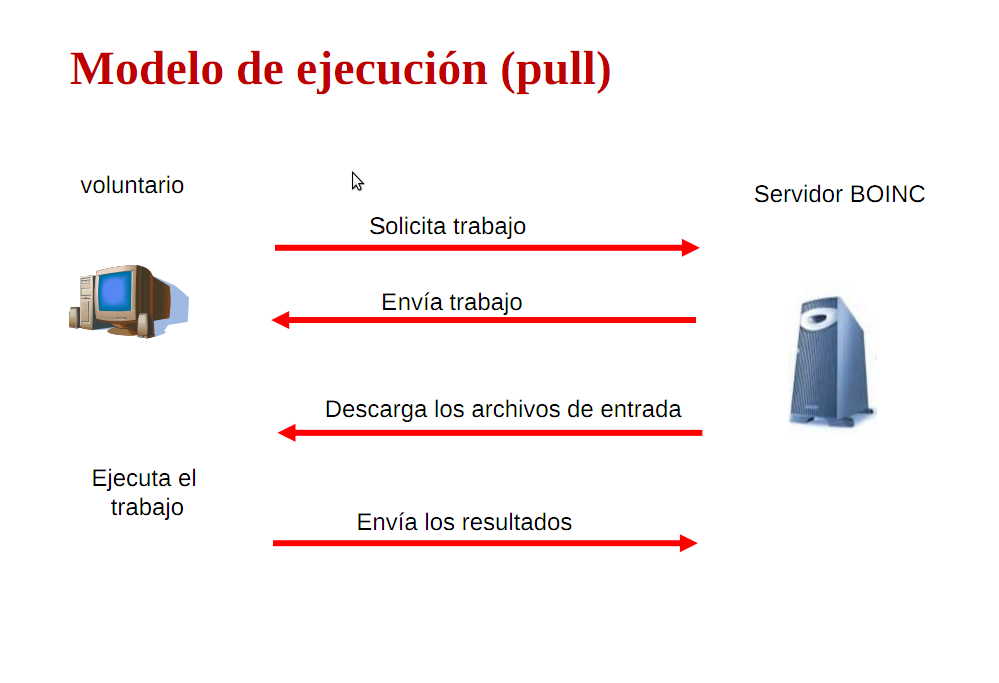
\includegraphics[height=3.5in,width=5.0in]{images/pull.png}
\caption{ Modelo de interacción cliente-servidor BOINC}
\label{fig:pull}
\end{center}
\end{figure} 

\subsection{Tolerancia a los hackers}

Los usuarios que colaboran con proyectos sobre computación voluntaria son anónimos por lo que sólo deben ingresan los datos típicos de una cuenta 
como alguna dirección de e-mail, país, etc. para poder participar. No hay control ni seguimiento de la forma en que el usuario colabora en el proyecto. 
Si entre ellos existen ciertos usuarios mal intencionados cuya meta es simplemente perjudicar el proyecto enviando resultados erróneo o pidiendo crédito 
por trabajos que no realizaron, éstos no pueden ser despedidos ni acusados. Es por eso que en los proyectos se deben tomar ciertos recaudos ante la 
posibilidad de tales malos comportamiento.  Uno de los métodos más utilizados es un sistema de firmas digitales, de tal manera que los hackers 
no pueden robar información. Un método para evitar resultados erróneos es enviar el mismo trabajo a dos máquinas diferentes y comparar resultados, 
de tal manera que estos y sus créditos sean aceptados si ambos se corresponden.

\subsection{Middleware para la computación voluntaria}

Las primeras aplicaciones para la computación voluntaria eran programas que combinaban una estructura para la computación científica y la computación
 distribuida con una arquitectura inflexible sobre la cual era muy complicado desarrollar nuevas aplicaciones o versiones.
En la actualidad, la computación voluntaria funciona a través de sistemas middleware quienes proveen una infraestructura para la computación distribuida. 
Sobre dichas infraestructuras es posible desarrollar proyectos con diversas metas como por ejemplo la investigación científica.

\vspace{4mm}

\textbf{Algunos de los middlewares más conocidos:}
\begin{itemize}
 \item \textit{BOINC}
 \item XtremWeb
 \item Xgrid
 \item Grid MP
\end{itemize}

Estos middlewares llevan un registro de los trabajos realizados por cada voluntario y los créditos que le corresponden por cada tarea computada. 
Generalmente, los créditos son tomados como una medida numérica sobre la cantidad de trabajos que ha realizado el cliente para un proyecto.

\subsection{Cómo contribuir}

Para que las personas puedan colaborar con un proyecto de computación voluntaria lo primero que deben hacer es descargarse la aplicación cliente desde 
la página del proyecto de acuerdo a la arquitectura y sistema operativo de su ordenador. Una vez descargada e instalada, el usuario deberá registrarse 
como nuevo cliente colaborador de uno o varios proyectos para quedar almacenado en su base de datos de modo que el servidor reconozca a su computadora
 como cliente. De esta manera, cuándo la computadora entre en estado ocioso, comenzará a comunicarse con el servidor para solicitar nuevos trabajos para
 computar.
En la cuenta mediante la cual el cliente se registró podrá ver estadísticas detalladas acerca de su participación como por ejemplo la cantidad de trabajos
 procesados, el número de unidades de trabajos completadas por hora y podrá comparar su contribución con la de otros clientes. Las estadísticas calculadas
 para cada cliente, créditos ganados y demás, se utilizan para generar una competencia sana entre los clientes de tal manera que se impulse a tener mayores
 y mejores voluntarios quienes compiten por estar en el ranking de los mejores contribuyentes.

\subsection{Evaluación de la computación voluntaria}

La computación voluntaria puede ser comparada con otros paradigmas de computación de alto rendimiento en ciertos aspectos:

\begin{itemize}

 \item \textbf{Rendimiento:} hay aproximadamente un millón de computadoras participando en lo que es computación voluntaria. 
			      Todas juntas suministran alrededor de 10 PetaFlops de poder computacional los cuales equivalen a billones de operaciones
			      de punto flotante por segundo. En comparación, la súper-computadora más rápida es de 1.4 PetaFlops y el mayor número de host 
			      que posee un grid es de decenas de miles. Si consideramos estos números, la computación voluntaria puede llegar a ser una
			      gran competencia para los demás paradigmas y tener el potencial para superarlos.

 \item \textbf{Costos y efectividad:} para las investigaciones científicas, la computación voluntaria es más barata que otros paradigmas. 
				      Proyectos de mediana escala en donde solo se necesitaría de un solo servidor,
				      gastaría aproximadamente 200.000 dólares al año,
				      mientras que un Clúster o Cloud-Computing tendría un costo significativamente mayor por el mismo rendimiento.

 \item \textbf{Política de asignación de recursos y la divulgación pública:} en paradigmas tradicionales de computación de alto rendimiento los
									    recursos son asignados por los organismos de financiación, instituciones,
									    comités. El público, a pesar de que paga por
									    los recursos, no tiene voz directa en su asignación y no sabe cómo están 
									    siendo utilizados. En la computación voluntaria, 
									    el público tiene un control directo sobre la asignación de recursos y sabe
									    lo que está siendo utilizado. Como resultado,
									    la conciencia pública sobre la ciencia es mayor y los proyectos de investigación
									    potencialmente pueden obtener importantes recursos de cómputo.

 \item \textbf{Adopción científica:} la computación voluntaria no ha sido ampliamente adoptada para los proyectos de investigación. 
				      Hay aproximadamente 60 grupos de investigación que están utilizando esta tecnología, a pesar de que centenares de grupos podrían 
				      beneficiarse de ella. Las tecnologías como Clústers o Grid son más utilizadas, en parte, porque los científicos han ignorado
				      a la computación voluntaria quizás debido a que no ofrece ni control directo de los recursos ni financiación del proyecto.
 
\end{itemize}

\newpage
\section{Berkeley Open Infrastructure for Network Computing  (BOINC)}

La Berkeley Open Infrastructure for Network Computing (BOINC) es un sistema middleware para la computación grid y voluntaria que trabaja bajo los términos de la licencia GNU Lesser General Public License (LGPL). Fue desarrollado por un equipo con sede en el Laboratorio de Ciencias en la Universidad de California, ubicada en Berkeley y dirigido por David Anderson.

En un principio el desarrollo de BOINC fue únicamente para dar soporte al proyecto SETI@home, pero éste nunca fue diseñado con altos niveles de seguridad por lo que usuarios mal intencionado intentaban ``engañar'' al proyecto enviando resultados falsos o tomando crédito por trabajos que no les correspondían. BOINC en parte fue desarrollado para combatir esos problemas de seguridad como una plataforma útil que a su vez permite dar soporte a otras aplicaciones distribuidas pertenecientes a distintas áreas de investigación tales como matemáticas, medicina, biología molecular, climatología, etc. 

El principal propósito del proyecto BOINC es hacer posible la investigación aprovechando el gran poder de procesamiento que las computadoras personales de todo el mundo pueden ofrecer en su conjunto.

Existen muchos proyectos independientes con diferentes propósitos que utilizan a BOINC, donde cada proyecto cuenta con su propio servidor, base de datos y aplicaciones; es decir, que no hay un directorio o proceso central de aprobación. 

Los usuarios pueden participar de varios proyectos a la vez. Ellos se encargan de controlar en cuales participar y cómo sus recursos son divididos entre dichos proyectos. Cuando un proyecto se cae o no posee más trabajos, sus recursos son divididos y reasignados a los demás proyectos en los que el usuario participa.

\subsection{Cliente BOINC}\label{boinc:manager}

El software BOINC client es la aplicación cliente que corre como demonio en las computadoras de los participantes, el cual provee y mantiene una comunicación directa con el servidor del proyecto y la plataforma local sobre la cual las aplicaciones van a ser ejecutadas.
\\
Sus principales funciones son:
\begin{itemize}
\item Se encarga de mantener una conexión, vía internet, entre cliente y servidor para intercambiar información, recibir trabajos y enviar resultados.
\item Se encarga de descargar y ejecutar los trabajos mediante la aplicación asociada a dicha tarea.
\item Determinar si la aplicación a descargar para el cómputo de una tarea es compatible con la arquitectura local del cliente. 
\item Si hay varias aplicaciones en ejecución, se encarga de planificar la distribución de los ciclos libres de la CPU entre dichas aplicaciones.
\end{itemize} 

El programa \textbf{BOINC Manager} ofrece una interfaz gráfica para monitorear y manejar una instancia del proceso boinc-client ya sea de manera local o manera remota. Básicamente ofrece una manera más simple y sencilla de poder manejar el cliente BOINC.

\subsection{Aplicaciones BOINC}

BOINC está diseñado para soportar aplicaciones que requieran grandes recursos computacionales y/o de almacenamiento por lo que cada proyecto puede obtener acceso a varios TeraFLOPS de poder computacional y varios TeraBytes de almacenamiento obtenidos de los participantes. 

Considerando que los proyectos BOINC obtienen recursos de voluntarios, para que las aplicaciones utilicen BOINC eficientemente deben cumplir las siguientes propiedades:

\begin{itemize}
\item \textbf{Atracción del público:} para ganar gran cantidad de participantes, las aplicaciones deben generar intereses en el público de tal manera que se sientan atraídos por participar en los proyectos. Por ello, es importante que los proyectos mantengan este interés creando, por ejemplo, un sitio web atractivo y generando gráficos interesantes en cada aplicación del proyecto.
\item \textbf{Paralelismo independiente:} la aplicación debe poder ser divisible en partes paralelas con poca o sin dependencia de datos.
\item \textbf{Baja transferencia de datos y tiempo de computación:} los datos de entrada y de salida de las aplicaciones son enviados por conexiones de internet comerciales por lo que las velocidades de transmisión podrían ser muy lentas. Como regla general, si una aplicación produce o consume más de un gigabyte de datos por día, sería recomendable utilizar otra tecnología en lugar de computación voluntaria ya que los tiempos de transferencia de datos de la aplicación, y posiblemente el tiempo de ejecución, podrían ser realmente altos para un ordenador de uso cotidiano.
\item \textbf{Tolerancia a fallos:} los resultados enviados por los voluntarios no pueden ser asumidos como correctos desde un principio, ya que pueden ser erróneos. La computación redundante puede ser utilizada para reducir la probabilidad de errores en un cierto porcentaje, pero no al 100\%. Que una aplicación tenga el 100\% de correctitud, podría indicar la existencia de un problema.
\end{itemize}

\subsection{Trabajos de BOINC}

La confección y manipulación de unidades de trabajos se encapsula bajo dos conceptos importantes dentro de BOINC: workunit y result. En su forma más amplia, una workunit, del lado del servidor, especifica una tarea que se debe realizar y los results representan instancias de esa tarea que serán enviados a clientes voluntarios para su computación.

\subsubsection{Workunit}

Una workunit describe y representa la tarea a ser computada por un cliente del proyecto. Cada workunit se asocia a una aplicación y a uno o varios archivos de entrada. Además, cuenta con diversos atributos que permiten brindar algunas características sobre el trabajo. Toda esta información se almacena en la base de datos del proyecto, más precisamente en la tabla workunit.
\\

\textbf{Atributos de una Workunit}
\\

Cada workunit está caracterizada por una serie de atributos que brindan información acerca del trabajo. A continuación se detallan algunos de ellos:

\begin{itemize}
\item \texttt{name}: es el nombre de la workunit. El nombre debe ser único entre todas las workunits del proyecto.
\item \texttt{application}: representa la aplicación que va a realizar esta computación. La workunit se asocia a una aplicación ya almacenada en la base de datos del proyecto, y no a una versión en particular. Si el formato de los archivos de entrada cambia y no es soportado por versiones anteriores de la aplicación, se deberá entonces liberar una nueva versión de la aplicación para todas las plataformas que se quiera soportar.
\item \texttt{input files}: representa una lista de archivos de entrada para un trabajo. Típicamente estos archivos son generados en el servidor, sin embargo si el elemento \texttt{<generate\_locally/>} está presente, el archivo es generado en por el cliente. 
\end{itemize}

Las workunits son configuradas por un archivo template que tiene la siguiente forma:
\newpage
\begin{lstlisting}[frame=shadowbox, language=xml, numbers=left, xleftmargin=8mm, framexleftmargin=22pt, basicstyle=\scriptsize, numberstyle=\footnotesize, breaklines=true, breakatwhitespace=false, captionpos=b, caption={Plantilla para la creación de una work unit.}, label=listing:boinc:wu:template, backgroundcolor=\color{gris}, keywordstyle=\color{Blue}]
<file_info>
    <number>0</number>
    [ <sticky/>, other attributes]
</file_info>
[ ... ]
<workunit>
    <file_ref>
        <file_number>0</file_number>
        <open_name>NAME</open_name>
    </file_ref>
    [ ... ]
    [ <command_line>-flags xyz</command_line> ]
    [ <rsc_fpops_est>x</rsc_fpops_est> ]
    [ <rsc_fpops_bound>x</rsc_fpops_bound> ]
    [ <rsc_memory_bound>x</rsc_memory_bound> ]
    [ <rsc_disk_bound>x</rsc_disk_bound> ]
    [ <delay_bound>x</delay_bound> ]
    [ <min_quorum>x</min_quorum> ]
    [ <target_nresults>x</target_nresults> ]
    [ <max_error_results>x</max_error_results> ]
    [ <max_total_results>x</max_total_results> ]
    [ <max_success_results>x</max_success_results> ]
</workunit>
\end{lstlisting}


\textbf{\\Estimaciones de recursos y límites}\\


Es importante que se provean valores precisos para los siguientes parámetros ya que éstos pretenden informar la cantidad y tiempo de uso que van a ocupar las workunits en los recursos del cliente.

\begin{itemize}
\item \texttt{rsc\_fpops\_est}: representan un número estimativo de cuantas operaciones de punto flotante va a requerir el trabajo para completarse. 
\item \texttt{rsc\_fpops\_bound}: representa un límite de operaciones de punto flotante que van a requerir los trabajos. Si este límite es superado, el trabajo es abortado.
\item \texttt{rsc\_memory\_bound}: el trabajo solo va a ser enviado a hosts con al menos esta cantidad disponible de memoria RAM. 
\item \texttt{rsc\_disk\_bound}: especifica un límite máximo de espacio en disco requerido por el trabajo, incluyendo todos los archivos de entrada, temporales, y archivos de salida. El trabajo será enviado a hosts con al menos esta cantidad de espacio en disco disponible.
\item \texttt{rsc\_bandwidth\_bound}:  si su valor no es cero, el trabajo será enviado solo a hosts con al menos esta cantidad de ancho de banda para la descarga. Es utilizado para trabajos con archivos de entrada de gran tamaño.
\end{itemize}

\textbf{\\Redundancia y atributos de scheduler}\\

\begin{itemize}
\item \texttt{delay\_bound}: representa el tiempo en segundos que debe pasar entre que se le envía un result al cliente y se recibe la respuesta. Si el tiempo que le toma al cliente completar la tarea y enviar el resultado excede este valor, el scheduler generará otro resultado para enviárselo a otro cliente. Si este atributo es seteado muy bajo, BOINC puede no ser capaz de enviar algunos results y su correspondiente workunit será seteada con error. Si se lo setea con un valor muy alto, puede haber un gran retraso en el servidor para obtener los resultado de vuelta.
\item \texttt{min\_quorum}: representa una mínima cantidad de resultados satisfactorios para un trabajo. La validación comenzará cuando haya esta cantidad de trabajos correctos. Generalmente se le asigna a este atributo 2 o más para hacer computación redundante.
\item \texttt{target\_nresults}: representa cuántos results se van a crear inicialmente. Éste debe ser al menos min\_quorum.
\item \texttt{max\_error\_results}: si el número de errores en el cliente excede este valor, la workunit es marcada como errónea; por lo cual no se crearán nuevos results y la workunit será asimilada. Esto se utiliza para prevenir a la aplicación cliente de workunits que causan fallos en la ejecución.
\item \texttt{max\_total\_results}: si el número de results para una workunit excede este valor, la workunit es marcada como errónea.
\item \texttt{max\_success\_results}: si el número de results satisfactorios excede este valor y el consenso para validar los results no se ha alcanzado, la workunit es marcada como errónea. Ésto se utiliza contra workunits que generan results no determinísticos.
\item \texttt{priority}: es opcional y se utiliza para darle prioridad a los trabajos. Los de prioridad más alta serán enviados primero.
\end{itemize}
\newpage
\textbf{\\Tipos de errores de una workunit}\\

Una workunit errónea, puede cumplir con alguna de las siguientes condiciones de error:

\begin{itemize}
\item \texttt{WU\_ERROR\_COULDNT\_SEND\_RESULT}: el scheduler no puede enviar la workunit a varios host, probablemente porque sus recursos exceden a la capacidad del cliente o porque no hay una versión de la aplicación para la plataforma de los hosts clientes. En dichos casos, BOINC no envía la workunit.
\item \texttt{WU\_ERROR\_TOO\_MANY\_ERROR\_RESULTS}: indica que se han retornado demasiados resultados erróneos para esta workunit. Es posible que estos errores se produzcan al descargar o subir archivos o bien por algún problema en la ejecución del cliente.
\item \texttt{WU\_ERROR\_TOO\_MANY\_SUCCESS\_RESULTS}: representa una excesiva cantidad de resultados satisfactorios que se han enviado sin consenso. Ésto indica que la aplicación puede ser no determinística.
\item \texttt{WU\_ERROR\_TOO\_MANY\_TOTAL\_RESULTS}: indica que se han enviado demasiados resultados para una workunit determinada.
\end{itemize}

Si alguno de estos errores persiste, BOINC cancela el envío de trabajos.

\subsubsection{Results}

Cada workunit tiene asociada uno o más resultados. Cada uno de ellos es una instancia de la unidad de trabajo original que se desea resolver. Precisamente son estos results los que son enviados a los clientes de BOINC para su posterior procesamiento.
En algunos casos pueden existir varias instancias o replicas de un result para una workunit dada. Los results quedan registrados en la base de datos del proyecto en la tabla \texttt{result}.

Una vez que todos los results asociados a una workunit han sido procesados e informados, el servidor BOINC seleccionará, mediante un proceso de validación y asimilación, el resultado más adecuado para convertirse en el resultado canónico. Una vez hecho ésto, la unida de trabajo se marca como completada.

Los results son configurados por una plantilla en formato XML:
\newpage
\begin{lstlisting}[frame=shadowbox, language=xml, numbers=left, xleftmargin=8mm, framexleftmargin=22pt, basicstyle=\scriptsize, numberstyle=\footnotesize, breaklines=true, breakatwhitespace=false, captionpos=b, caption={Plantilla para la configuración de un result.}, label=listing:boinc:result:template, backgroundcolor=\color{gris}, keywordstyle=\color{Blue}]
<file_info>
    <name><OUTFILE_0/></name>
    <generated_locally/>
    <upload_when_present/>
    <max_nbytes>32768</max_nbytes>
    <url><UPLOAD_URL/></url>
</file_info>
<result>
    <file_ref>
        <file_name><OUTFILE_0/></file_name>
        <open_name>result.sah</open_name>
    </file_ref>
</result>
\end{lstlisting}


\textbf{\\Atributos de un result}\\

Los atributos principales de cada result son por un lado el nombre que permite su identificación, especificado por el tag \texttt{<name>} en el template, y por otro lado la lista de nombres de archivos de salida donde se escriben los resultados de la computación. En la plantilla se distinguen con el tag \texttt{<file\_name>} dentro de \texttt{<file\_ref>}.\\

Otros atributos:

\begin{itemize}
\item \texttt{<OUTFILE\_n>}: es reemplazado con un string de la forma \texttt{wuname\_resultnum\_n} donde wuname es el nombre de la workunit a la cual el result está asociado y resultnum es el número de result. El \texttt{n} se utiliza como numeración de cada tarea.
\item \texttt{<generate\_locally>}:  genera los archivos de entrada de la tarea en el cliente.
\item \texttt{<url>}: se especifica la url donde se deben subir los resultados.
\end{itemize}

\subsection{Conceptos básicos}

En esta sección se presentan de manera introductoria conceptos importantes de los que se hablará a lo largo de los capítulos.

\subsubsection{Aplicaciones y sus versiones}

Un proyecto BOINC puede contar con un número ilimitado de aplicaciones las cuales son registradas en la base de datos del proyecto. A su vez cada aplicación puede contar con varias versiones e incluso estar disponible para diferentes plataformas. Esto último se debe a que generalmente un nuevo cambio produce una nueva versión de la aplicación.
La tabla \texttt{app} de la base de datos es la encargada de almacenar los datos de una aplicación, y la tabla \texttt{app\_version} de registrar las diferentes versiones.

\subsubsection{Plataforma}

Una plataforma especifica un tipo de destino sobre el cual va a correr una aplicación BOINC. Típicamente se representa mediante la combinación de la arquitectura de CPU y el sistema operativo. 

Cada versión de una aplicación está asociada a una plataforma. Si una aplicación no cuenta con una versión para la plataforma de un determinado cliente, el scheduler de BOINC no enviará trabajos a dicho cliente.

Una aplicación compilada para una plataforma determinada debe tener la siguiente estructura como nombre de archivo:\\
\texttt{appName\_1.0\_platform}\\
donde \texttt{appName} indica el nombre de la aplicación, \texttt{1.0} representa la versión del programa y \texttt{platform} especifica la plataforma asociada al ejecutable.

BOINC incluye un conjunto de plataformas estándares en sus proyectos y que por defecto vienen cargadas en el archivo de configuración del proyecto.

\subsubsection{Cuentas de usuarios}

Toda persona que desea colaborar con un proyecto BOINC debe registrarse por única vez en dicho proyecto indicando una dirección de e-mail y una contraseña. Una vez hecha la registración de la cuenta automáticamente el usuario quedará asociado al proyecto para comenzar con su colaboración.

Cada cuenta puede a su vez estar asociada con diferentes host. Es decir que un usuario podría colaborar utilizando la misma cuenta desde diferentes ordenadores.

\subsubsection{Unirse a un proyecto}

Toda persona que quiera colaborar con un proyecto debe descargarse el \textit{cliente BOINC} de su sitio oficial \footnote{\url{http://boinc.berkeley.edu/}} el cual se encuentra disponible para las diversas plataformas tales como Microsoft Windows, Mac OS X y Linux.

Una vez descargado e instalado BOINC Manager, la unión a un proyecto solo requiere colocar la url del proyecto y crear una cuenta en ese proyecto en caso de no contar con una.

Mediante esta aplicación se puede estar adheridos a varios proyectos e incluso configurar cómo colaborar con cada proyecto y en qué momentos estar disponibles para la computación y descargas de trabajos.

Si un ordenador está adherido a múltiples proyectos, sus recursos disponibles se dividen entre ellos en proporción a los requerimientos de cada uno.

\subsection{Proyecto BOINC}

Un proyecto BOINC es el encargado de administrar todo el proceso de computación distribuida. Permite la administración de cuentas de usuarios, aplicaciones, estadísticas e incluso configurar cómo van a ser distribuidos los trabajos.

Cada proyecto está conformado por un servidor de bases de datos, un sitio web, demonios en ejecución y un conjunto de aplicaciones encargadas de generar las tareas que luego será distribuidas por BOINC. 

El sitio web del proyecto es utilizado para informar al público en general sobre las tareas realizadas por la organización con el propósito de aumentar la cantidad de voluntarios. Además, ofrece una interfaz donde el usuario puede configurar los datos de su cuenta.

Todo proyecto se identifica por la URL de su sitio web mediante la cual los usuarios se adhieren voluntariamente utilizando la aplicación cliente \textit{BOINC Manager}. 

\subsubsection{Características de los proyectos}

BOINC provee ciertas características que simplifican la creación y  el funcionamiento de los proyectos:

\begin{itemize}
\item \textbf{Framework de aplicaciones flexible}: aplicaciones escritas en lenguajes regularmente conocidos como C, C++ o Fortran pueden correr como una aplicación de BOINC. Sólo hacen falta pequeñas modificaciones para que puedan formar parte de los proyectos.
\item \textbf{Seguridad}: BOINC protege los proyectos contra distintos tipos de ataques. Por ejemplo, utiliza sistema de firmas digitales basado en encriptación de claves publicas para proteger contra la distribución de virus.
\item \textbf{Múltiples servidores y tolerancia a fallos}:  los proyectos pueden tener varios servidores de datos y varios servidores de scheduling por separado, cada uno encargándose de sus correspondientes tareas. Si alguno de estos servidores se cae, los clientes automáticamente prueban alternar a otro servidor. Si todos los servidores están caídos, los clientes realizan un retroceso exponencial de sus requerimientos para evitar saturar los servidores cuando vuelvan a funcionar.
\item \textbf{Disponibilidad del código fuente}: BOINC es distribuido bajo la licencia LGPL. Sin embargo, las aplicaciones no necesitan ser “open source”.
\item \textbf{Soporte de grandes volúmenes de datos}: BOINC soporta aplicaciones que producen o consumen gran cantidad de datos o que usan gran cantidad de memoria. La distribución de los datos puede propagarse por varios servidores y los participantes del proyecto pueden transferir grandes volúmenes de datos discretamente. Los trabajos solo son enviados a hosts que tienen la capacidad de manejarlos.
\end{itemize}

\subsubsection{Servidor}

El servidor de BOINC engloba todas las herramientas, aplicaciones y demonios que permiten crear, enviar y administrar workunits y results, entre otras cosas. Puede correr en una o varias máquinas, lo que le permite a BOINC ser fácilmente escalable a proyectos de cualquier envergadura. 

El servidor BOINC corre sobre computadoras basadas en Linux y usa Apache, PHP y MySQL como bases para su interfaz web y base de datos respectivamente.

Dentro de BOINC, podemos considerar diferentes clases de servidores \linebreak dependiendo del rol que cumpla. Cabe destacar que un solo servidor BOINC cumple con todos los roles, pero en ocasiones y por necesidad de optimizar, se pueden tener varios servidores cumpliendo un rol especifico:

\begin{itemize}
\item \textbf{Data Server}: es la porción del sistema BOINC que se encarga de enviar a los participantes los datos necesarios para procesar las workunits.
\item \textbf{Scheduling Server}: se encarga de coordinar los trabajos generados para hacer el mejor uso de los recursos disponibles a la hora de enviar los trabajos a procesar.
\item \textbf{Database Server}: actúa como un repositorio manteniendo una estructura relacional de información en la base de datos del proyecto.
\item \textbf{File Server}: actúa como un repositorio de información almacenada en archivos del proyecto BOINC. Este repositorio es usualmente desestructurado, hasta el punto que se llegan a perder archivos. Los únicos elementos estructurados son los nombres de archivos y carpetas.
\end{itemize}

\subsubsection{Configuración de un proyecto}
\label{seccion:boinc:config:xml}
La configuración de los proyectos BOINC se encuentra definida por un archivo de configuración llamado \texttt{config.xml} situado en el directorio raíz del proyecto. Este archivo es creado con valores por defecto cuando se crea un nuevo proyecto. Sin embargo, será necesario agregar o modificar algunos valores durante la vida del proyecto para así optimizar y adaptar a las necesidades de cada organización.

Para más detalles de cómo crear y administrar proyectos puede consultar la documentación oficial de BOINC\footnote{\url{http://boinc.berkeley.edu/trac/wiki/ProjectMain/}}.

\subsubsection{Scheduler}

El scheduler de BOINC se encarga de administrar la distribución de trabajos entre todos los clientes conectados al proyecto tratando de hacer el mejor uso de los recursos disponibles. El scheduler es quien determina qué trabajos van a ser enviados o recibidos desde o hacia los clientes. 

El scheduler es un proceso que puede correr en un sólo servidor dedicado o bien puede ser combinado con otros procesos o demonios del sistema BOINC en un mismo servidor. Si este demonio no está funcionando, el sistema BOINC queda obsoleto.

El scheduler en sí es una instancia de un script CGI o Fast-CGI el cual se crea en el momento en que el servidor recibe un requerimiento del cliente, como por ejemplo solicitar workunits, reportar trabajos completados, actualizar preferencias de base de datos, etc.

\subsection{Interacción cliente-servidor}

En esta sección se dará una visión general sobre cómo interactúa el servidor BOINC con los clientes conectados. Considerando el caso donde el cliente ya se encuentra adherido al proyecto, la interacción cliente-servidor se manifiesta de la siguiente manera:

\begin{enumerate}
\item En primer lugar, cuando un cliente se conecta recibe el archivo maestro del proyecto y un conjunto de tareas enviadas por el scheduler. Estas tareas dependen de los recursos con los que cuente el ordenador del cliente. El servidor no le asignará tareas que requieran más recursos de los que dicha máquina posee.
\item El cliente descarga el ejecutable y los archivos de entrada de la aplicación desde el servidor. Si el proyecto libera una nueva versión de la aplicación, el ejecutable se descarga de manera automática.
\item Una vez que el cliente haya descargado los archivos del punto anterior, ejecuta la aplicación generando archivos como salida. Si la ejecución de la tarea falla por algún motivo en particular, en caso de existir, automáticamente se vuelve a descargar una réplica de dicha tarea para intentar nuevamente.
\item Una vez finalizado, el cliente sube los archivos de salida al servidor.
\item Por último, el cliente reporta las tareas completadas al scheduler para solicitar nuevas tareas.
\end{enumerate}

La figura \ref{fig:how-boinc-works} muestra en resumen los puntos mencionados.

\begin{figure}[H]
	\begin{center}
  		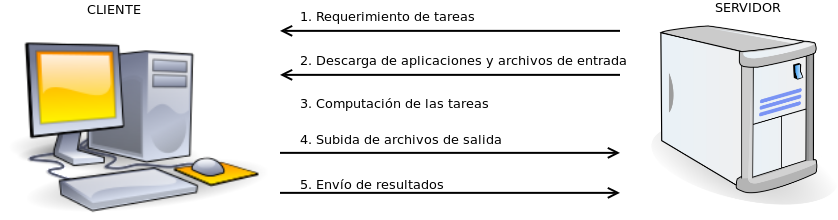
\includegraphics[scale=0.45]{images/how-boinc-works.png}
		\caption{Interacción entre cliente y servidor}
		\label{fig:how-boinc-works}
		\end{center}
\end{figure} 

El requerimiento que un cliente envía al servidor para solicitar trabajos consiste de un archivo XML en donde se detalla toda la información de hardware, de disponibilidad y a su vez se incluye el requerimiento de nuevos trabajos. En el caso de que se hayan completados trabajos, también se incluye la lista de dichos trabajos. 

Cuando el servidor responde el requerimiento, envía al cliente un mensaje de que incluye una lista de nuevos trabajos especificados mediante un elemento XML que lista la aplicación, los archivos de entrada y salida, y un conjunto de servidores desde dónde cada archivo puede ser descargado.

\subsection{Entrega de créditos}

El servidor del proyecto mantiene un registro sobre cuántos trabajos ha computado cada cliente; este registro es llamado \textit{créditos}. Básicamente según la cantidad de trabajo que ha realizado el cliente el servidor le otorga una cierta cantidad de créditos como bonificación.

La mayoría de los proyectos BOINC manejan el sistema de créditos de la siguiente manera:

\begin{itemize}
\item Cada tarea puede ser enviada a dos o más computadoras. El proyecto hace esto para comparar los resultados de cada tarea y verificar que no se estén enviando resultados erróneos.
\item Cuando los clientes reportan los resultados, estos reclaman cierto monto de créditos basado en la cantidad de tiempo de CPU que fue utilizado para procesar el trabajo
\item Cuando al menos dos resultados fueron reportados, el servidor los compara y si éstos se corresponden se le asigna a cada usuario el mínimo monto de créditos reclamado por alguno de ellos.
\end{itemize}

\subsubsection{Créditos vía Trickle Messages}

Los Trickle Mesagges permiten que las aplicaciones puedan comunicarse con el scheduler durante la ejecución de una workunit. Éstos pueden ir en cualquier dirección: los Trickle-Up son mensajes que van desde la aplicación cliente al scheduler y los Trickle-Down son los que toman el sentido contrario.

Este mecanismo tiene los siguientes usos:\\

Para solicitar créditos parciales:
\begin{itemize}
\item La aplicación cliente envía un mensaje trickle-up conteniendo su actual uso de CPU, así el usuario puede obtener créditos parciales.
\item El scheduler envía un mensaje Trickle-Down conteniendo el crédito total que posee hasta el momento el usuario.
\end{itemize}

Para verificar estado:

\begin{itemize}
\item La aplicación cliente envía un mensaje trickle-up conteniendo un resumen de su estado de ejecución, así el scheduler puede decidir si la computación debe ser abortada o debe continuar.
\item El scheduler envía un mensaje Trickle-Down diciéndole a la aplicación que aborte.
\end{itemize}

\subsection{Demonios de BOINC}

En el contexto de la informática, un demonio es un programa que realiza cierta tarea específica y se ejecuta en segundo plano, en lugar de estar bajo el control directo del usuario. 

En el caso de BOINC, los demonios son programas que forman parte del servidor y cumplen con diferentes roles dentro del proyecto.

\subsubsection{Demonios para el manejo de trabajos}

El manejo y distribución de trabajos en un proyecto BOINC incluye ciertos demonios los cuales son independientes de la aplicación que se esté ejecutando.

\textbf{\\Work Generator}: es uno de los componentes del núcleo del sistema BOINC. Está diseñado para crear workunits y results que se emitirán a los participantes para ser procesados. Su tarea consiste en crear los trabajos y organizar sus archivos de entrada para luego enviarlos a los clientes.

\textbf{\\Feeder}: mantiene una conexión directa con la base de datos y se encarga de crear un segmento de memoria compartida utilizado para transferir registros de la base de datos al scheduler.
 
Cuando un cliente realiza una conexión con el scheduler, este demonio se encarga de aislar al scheduler de la base de datos y conectarlo a esta última. De esta manera se le quita al scheduler la carga de mantener una conexión directa con la base de datos.

\textbf{\\Transitioner}: su función es manejar los estados de transición de las workunits y results. Se encarga de verificar continuamente si las workunits están listas para ser enviadas o si algún result fue recibido.
Cuando una workunit es creada, el transitioner se encarga de crear los results iniciales en la tabla result para dicha workunit. Si la ejecución de la workunit falla, este demonio creará nuevos results para reintentar la ejecución. Cuando los resultados son enviados nuevamente al servidor, el transitioner los toma para actualizar el estado de los mismo en la base de datos. Luego de actualizar su estado, este demonio crea un conjunto de resultados que son marcados como “listos para validar” que luego serán tomados por el demonio Validator.

\subsubsection{Demonios para el manejo de resultados}
\label{seccion:demonio:validator}
\textbf{\\Validator}: como el nombre lo indica, este demonio se encarga de hacer la validación de los resultados enviados por los clientes para determinar si son correctos o no. Se debe tener un validator por cada aplicación que se vaya a ejecutar en el proyecto. Este demonio solo va a considerar resultados correspondientes a aquellas unidades de trabajo cuyo flag \texttt{NEED\_VALIDATE} esté activo. 

Además, es el encargado de asignar créditos a los usuarios por sus trabajos realizados.

Luego de que los resultados de una workunit pasan por este demonio, de todos ellos se obtiene un solo resultado válido denominado \textit{resultado canónico}.

\textbf{\\Assimilator}\label{boinc:assimilator}: este demonio se encarga de tomar los trabajos completados para realizar determinadas tareas luego de que el demonio Validator determine si encontró el resultado Canónico para una workunit, o bien la marcó como errónea. 

Las tareas a realizar por el assimilator suelen ser específicas de la aplicación. Para workunits validadas correctamente, estas tareas podrían consistir en copiar los archivos de salida desde el directorio “upload” a otro directorio permanente, o llegar a analizar el archivo de salida y registrar nueva información en la base de datos, o bien generar nuevas workunits. Para workunits erróneas, generalmente se genera una salida en un archivo informando el error.

\subsubsection{Demonios para la limpieza del proyecto}

\textbf{\\File Deleter}: es el encargado de limpiar todos los archivos de workunits y results que el proyecto ya no necesita. Básicamente se encarga de eliminar los archivos de los directorios upload y download que fueron utilizados para realizar determinadas tareas que ya cumplieron su ciclo y fueron finalizadas. 

\textbf{\\Database Purge}: este demonio se encarga de eliminar los registros de la base de datos para mantenerla lo más pequeña posible y así no alterar el rendimiento de las consultas.

Si consideramos la manera en que el proyecto trabaja, el tamaño de las tablas de workunit y results se incrementa significativamente. Para evitar que ésto ocurra, BOINC provee el demonio \texttt{db\_purge} el cual mueve los registros de las tablas workunit y result a un archivo XML que será almacenado en el directorio \texttt{archive/} creado por el mismo demonio. Los registros de la tabla workunit son eliminados solo cuando sus archivos de entrada hayan sido eliminados.


\section{FuD}
\label{seccion:fud}

\subsection{¿Qué es FuD?}

FuD es un framework para automatizar la implementación de aplicaciones distribuidas. El uso de FuD no depende del problema que se quiera implementar y tampoco 
obliga a utilizar un modelo de comunicación en particular. Por consiguiente, las aplicaciones FuD pueden correr en clústers heterogéneos y dinámicos. 
Es decir, que el procesamiento en los clientes puede variar de acuerdo al hardware y software con el que se cuente. Por ejemplo, uno podría contar con muchas 
combinaciones de sistemas operativos y arquitecturas de hardware corriendo simultáneamente, además, el hecho de que el clúster sea dinámico significa que el procesamiento
 de los clientes puede fallar en un momento dado, que su disponibilidad no es fiable y que incluso pueden desconectarse sin previo aviso o bien, nuevos clientes pueden
 conectarse durante la ejecución de la aplicación.

En sí, FuD es sólo una implementación parcial de una librería si el middleware de distribución por defecto, \textit{boost::asio}, es quitado. Sin embargo, este middleware se
 incluye con la distribución de FuD y por lo tanto el framework puede compilarse como una librería. Una versión compilada de FuD consta de una librería para la distribución de
 trabajos utilizando un middleware de distribución en particular. Las librerías que surjan de compilar con diferentes middlewares de distribución deberían funcionar sin problemas,
 siempre y cuando la disponibilidad de clientes no sea un problema para algún middleware. Esto último significa que el mismo problema puede ser resuelto en diversos clústers de ordenadores, hasta en una simple computadora ejecutando la aplicación cliente y servidora juntas.

Es importante tener en cuenta que las diferentes implementaciones de middleware deberían beneficiar a los clústers que cuenten con el mismo diseño 
para el cual el middleware fue diseñado. Por ejemplo, MPI es más adecuado para clústers de ordenadores interconectados localmente mediante una vía rápida.
 Por el contrario, BOINC ofrece una capacidad de procesamiento mucho mayor a pesar de aumentar el costo de comunicación vía Internet.
Organizaciones sin fines de lucro en la mayor parte de los casos no disponen de grandes capacidades de procesamiento y por lo que generalmente dependen de
 los diferentes tipos de contribuciones recibidas para así poder manejar sus necesidades computacionales.


\subsection{¿Cómo funciona una aplicación FuD?}

En su sentido más amplio, FuD se divide en dos aplicaciones: el servidor y el cliente. Para cualquier proyecto FuD, debe existir exactamente 
un servidor con uno o varios clientes conectados a él. 

El servidor y sus clientes mantienen una relación master-worker por lo que el servidor es 
el encargado del progreso general del sistema y los workers (clientes) son los encargados de realizar el procesamiento de datos.

\subsubsection{Clientes de procesamiento}

Un cliente de procesamientos, conocido en FuD como \texttt{ClientProcessor}, es un nodo de procesamiento conectado al servidor.
 Los clientes de procesamiento pueden tomar muchas formas y tener capacidades de cómputos muy diferentes, por lo que no deben hacerse
 suposiciones de cuán rápido un cliente puede resolver un trabajo, de su disponibilidad o de cualquier otra característica.

La única tarea de un cliente de procesamiento es esperar por un mensaje proveniente desde el servidor el cual contendrá encapsulado 
algún trabajo que necesita ser realizado. 

Cada cliente de FuD es independiente de los demás clientes, por lo que desconoce cómo afectará este trabajo al resto del sistema.
Cuando el cliente recibe un mensaje desde el servidor, éste debe procesarlo y una vez finalizado debe informa el resultado obtenido de la computación al servidor.
La figura \ref{fig:Client-Server} muestra un servidor corriendo una aplicación llamada The clusterer que utiliza la librería FuD con la implementación asincrónica de E/S (\texttt{ASIO}\footnote{Asio es una librería de código abierto, desarrollada en C++ para la comunicación en red. Ésta provee a los desarrolladores un consistente modelo de E/S asincrónico utilizando el enfoque moderno de C++.}) perteneciente a la librería \texttt{Boost} para manejar las conexiones de la capa de comunicación del framework.

\begin{figure}[H]
\begin{center}
  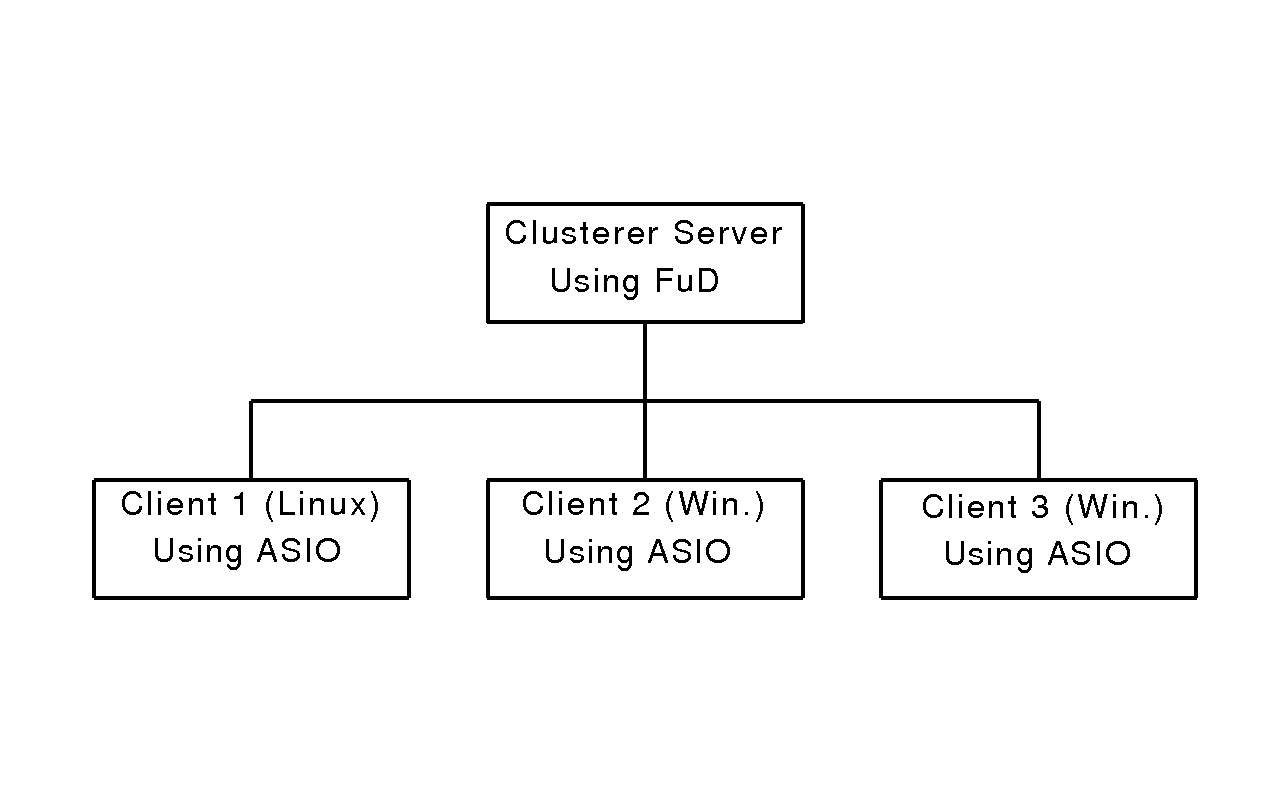
\includegraphics[height=3.5in,width=5.0in]{images/FuD-fig1.png}
\caption{Muestra tres clientes conectados al servidor}
\label{fig:Client-Server}
\end{center}
\end{figure} 

En este caso, hay dos tipos de sistemas operativos diferentes conectados al servidor.

\subsubsection{Trabajos distribuidos}

Un \texttt{DistributableJob} es un concepto de trabajo abstracto que encapsula cualquier trabajo que será realizado. No existe un límite para la cantidad y tipos
 de trabajos distribuibles que pueden ser creados. 

Es posible que un proyecto complejo requiera de diferentes tipos de trabajos distribuibles,
 donde cada uno de ellos tendrán varias instancias para diferentes casos.

La propiedad más importante de estos trabajos a gran escala es que ellos pueden ser subdivididos en tareas más pequeñas llamadas \texttt{JobUnits},
 donde cada una de ellas representa una computación concreta que será llevada a cabo por alguno de los nodos de procesamiento.

Las \texttt{JobUnits} generadas por un \texttt{DistributableJob} tienen dos características importantes:
\begin{enumerate}
 \item  A pesar que la generación se da en un orden determinado, no debe ser un requerimiento el orden en cómo las job units son computadas.
\item  Dos \texttt{JobUnits} no deben representar la misma computación.
\end{enumerate}

Por lo tanto, la relación entre trabajo distribuible y unidad de trabajo es que este último es una sub-tarea del primero. Solo existen dos niveles de subdivisión 
por lo que una job unit no puede ser sub-dividida en tareas más pequeñas. Considerar el ejemplo de la figura \ref{fig:example} donde se muestra cómo se puede construir una aplicación
 para realizar la sumatoria de la suma de N vectores. Supóngase que  se tienen vectores de 1 hasta N donde cada uno tiene una cantidad variable de elementos y se quiere calcular
 la sumatoria de la suma de todos los elementos en cada vector.

  Es fácil ver que solo se necesita de un solo trabajo distribuible: uno que pueda llevar a cabo la suma de los elementos
 de un vector. Luego, este mismo \texttt{DistributableJob} es re usado para calcular la suma de los resultados parciales obtenidos y almacenados en el vector temporal T.

Es importante destacar que aquí existen diversas posibilidades de sincronización, pero aquí elegimos una simple:

\begin{enumerate}
 \item  Los pasos 1 y 2 se ejecutarán de manera concurrente. En cualquier momento dado, todos los clientes conectados podrían estar procesando secciones diferentes de diferentes vectores.
\item El paso 3 se realizará una vez que los \texttt{DistributableJobs} de 1 a N estén completos. En este punto, el vector T contendrá los resultados parciales necesarios para llevar
 a cabo la suma del último vector. Por lo tanto, en ese momento se crea un nuevo trabajo distribuible N+1 el cual resuelve la sumatoria de todos los elementos de T. Cuando
 este \texttt{DistributableJobs} finalice, habremos obtenido la suma total de todos los vectores disponibles.
\end{enumerate}


\begin{figure}[H]
\begin{center}
  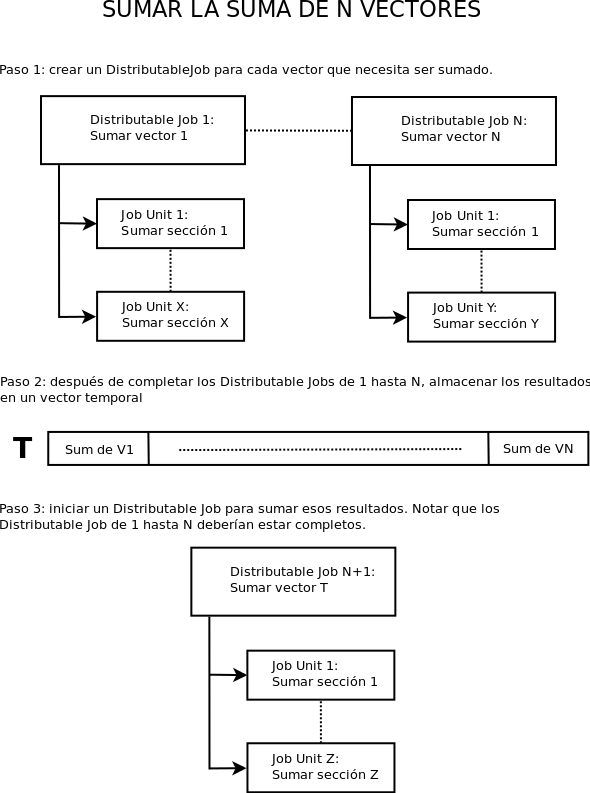
\includegraphics[height=7.5in,width=5.0in]{images/FuD-fig2.png}
\caption{Muestra el proceso de sumar N vectores}
\label{fig:example}
\end{center}
\end{figure} 


\subsubsection{Unidades de Trabajo}

Una \texttt{JobUnit} es un trabajo abstracto que encapsula el concepto de una tarea simple que será realizada. 
Una \texttt{JobUnit} es atómica por lo que no puede subdividirse en otras unidades de trabajo. La tarea en sí debe ser representada por un mensaje,
 el cual será pasado a un cliente de procesamiento quien se encargará de computarla.
Una característica importante de las \texttt{JobUnits} es su tamaño. Existen dos maneras de observar su tamaño: uno es el definido por el problema de la aplicación,
y el otro es el tamaño en bytes del mensaje que lleva.

Los tamaños de las \texttt{JobUnits} pueden variar por muchas razones, sin embargo es importante considerar algunas reglas en su generación:
\begin{enumerate}
\item Su tamaño en bytes no debería ser muy grande ya que podría obstruir un canal de comunicación utilizado.
\item  El tamaño del problema no debería ser muy grande de lo contrario los clientes de procesamiento podrían necesitar una cantidad de tiempo irrazonable para resolver la tarea.
\item  La combinación de estas dos nociones de tamaño debe darse de tal manera que el tiempo para comunicar el mensaje sea inferior al tiempo necesario para el procesamiento de la tarea. 
El objetivo de ésto es minimizar el tiempo total de computación consumido por un proyecto dado. 
\end{enumerate}

En el ejemplo dado en el diagrama de la figura \ref{fig:example} el único tipo de unidad de trabajo es el que puede sumar una serie de elementos.
 En este caso, el mensaje será una secuencia numérica en sí y el mensaje de retorno será un simple número que representará el resultado de la suma de esa sección.
En el caso del diagrama de la figura \ref{fig:example}, un vector pequeño podría producir solamente una simple \texttt{JobUnit} que encapsule la suma del vector entero.

\subsubsection{Manejador de Clientes}

El \textit{ClientsManager} es el modulo encargado de manejar la registración y disponibilidad de clientes de procesamiento. La figura \ref{fig:Client-Server}
 muestra un posible estado del modulo donde hay 3 clientes de procesamiento conectados. El manejador de clientes puede tener diferentes implementaciones que se adapten a diferentes diseños de clústers.\\
Por defecto, FuD se provee con la implementación asincrónica de E/S (\textit{ASIO}) de Boost para manejar las conexiones de la capa de comunicación del framework.
El propósito de esta tesis es proveer de una nueva implementación de este modulo que permita a las aplicaciones desarrolladas con FuD
 entrar en el mundo de la computación distribuida y voluntaria brindada por BOINC.

\subsubsection{Manejador de Trabajos}

El eje central para la gestión de \texttt{DistributableJobs} y \texttt{JobUnits} de la aplicación servidora es el \texttt{JobManager}. Éste es el encargado de
 administrar estos dos tipos de trabajos al mismo tiempo que mantiene comunicaciones con el \texttt{ClientsManager} con el fin de maximizar el uso de los recursos disponibles en un momento dado.

\subsubsection{La aplicación principal}

Para unificar todos estos conceptos, el desarrollador de la aplicación debe implementar instancias de \texttt{DistributableJob} y utilizarlas en la aplicación principal.

\subsection{Diseño de FuD}

Como se mencionó al comienzo de esta sección, el diseño de FuD se divide en dos partes, cliente y servidor donde cada una de ellas se encuentra organizada en
 tres capas bien definidas. Cada una de ellas tiene una funcionalidad clara y específica.

La comunicación entre las capas es estrictamente limitada ya que existe un solo punto de comunicación con la capa del anterior o del siguiente nivel.

Cuando un mensaje es creado, éste debe atravesar las diferentes capas comenzando desde la de nivel más alto hacia la capa inferior, y luego recorrer en
 sentido contrario las capas del lado receptor. Ver la figura \ref{fig:FuD-Design}.


\begin{figure}[H]
\begin{center}
  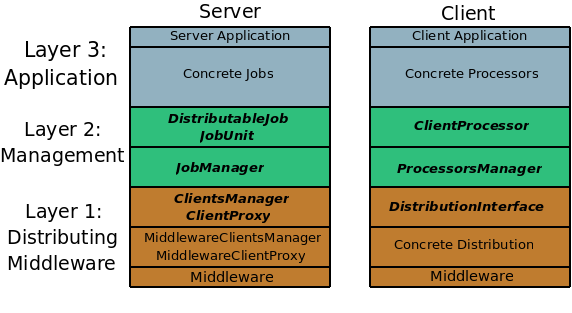
\includegraphics[height=3.5in,width=5.0in]{images/FuD-diseno.png}
\caption{Capas del framework FuD }
\label{fig:FuD-Design}
\end{center}
\end{figure} 


\subsubsection{Capa de aplicación (L3)}

Esta capa proporciona los componentes que contienen todos los aspectos del dominio del problema a resolver. Dichos aspectos incluyen todas las definiciones
 de datos y sus tratamientos correspondientes como así también todos los algoritmos relevantes para la resolución del problema en cuestión.
Por estos motivos, esta capa no es, en algún sentido, considerada como parte de FuD. La implementación de una aplicación que usa la librería,
 no es parte de la librería. Sin embargo, su inclusión es una ayuda valiosa para la comprensión de cómo funciona FuD.

Es necesario que del lado del servidor se implemente la aplicación principal, la cual hará uso de una simple interfaz en la abstracción de un trabajo distribuible permitiendo así codificar la estrategia de distribución de trabajos.
Del lado cliente, solo se necesita implementar los métodos encargados de realizar las computaciones indicadas por una unidad de trabajo.

\subsubsection{Capa de administración de trabajos (L2)}

La responsabilidad de esta capa es el manejo de trabajos, lo cual incluye la creación de instancias de \textit{DistributableJobs}
 y el pedido de generación de \texttt{JobUnits} las cuales van a ser entregadas a la capa inferior para su procesamiento. Una vez que la tarea finalice, se debe informar a las capas superiores de la tarea completada y los resultados obtenidos.

\subsubsection{Capa de distribución (L1)}

En el lado del servidor, la registración de clientes y sus estados es manejado por esta capa. 

Tanto del lado cliente como del servidor, la parte fija está dada por interfaces. Las implementaciones concretas de este nivel son variables
 y están determinadas por el middleware a utilizar, por ejemplo \textit{Boost.Asio}, \textit{MPI} o \textit{BOINC}.  

Desde esta vista abstracta de diseño, es importante destacar que la capa \textbf{L1} constituye por sí sola un particular esquema de manejo de clientes. Éste podría implementarse usando threads o procesos en un simple núcleo, una \textit{API} de memoria distribuida como \textit{MPI} o, como en el caso de esta tesis, computación voluntaria a través de internet utilizando BOINC.

Estas implementaciones separadas deberían poder intercambiarse sin ningún problema. Utilizar cualquiera de las implementaciones de esta capa no debe afectar la resolución del problema que se intenta resolver, por lo que los resultados obtenidos deben ser los mismos.
Debe notarse que en todo el sistema el tiempo total de cálculo de una unidad de trabajo en un entorno ideal está dado por varios factores:\\

T$_{job−unit}$ = T$_{send}$ + T$_{compute}$ + T$_{receive}$ + T$_{handle−results}$

\vspace{5mm}

T$_{send}$ y T$_{receive}$ dependen de la comunicación, T$_{receive}$ depende de la arquitectura del cliente y T$_{handle−results}$ depende del servidor. 

El tamaño de una unidad de trabajo debe minimizar esta ecuación. Si un usuario contara con un solo núcleo de procesamiento y por ejemplo
 usara threads las variables de tiempos T$_{send}$  y T$_{receive}$ serían nulas mientras que las dos restantes se incrementarían por el costo de mantener varios threads en ejecución.  


\section{El lenguaje de programación C++}

\textit{C++} es un lenguaje de programación desarrollado en el año \textit{1979} por \textsc{Bjarne Stroustrup} en los laboratorios \textsc{Bell}. 
Inicialmente era llamado \textit{“C con clases”} ya que se presentaba como una mejora o extensión del lenguaje de programación \textit{C}. 
Los contenidos más completos sobre este lenguaje se los pueden encontrar en el propio libro de Bjarne Stroustrup \cite{cplusplus}.\\

\textit{C++} es un lenguaje multi-paradigma y estáticamente tipado. Es considerado un lenguaje de nivel medio, ya que comprende características de lenguajes de alto y bajo nivel.\\

Este lenguaje fue elegido como lenguaje de implementación del framework FuD ya que éste permite el uso de técnicas orientadas a objetos y produce eficiente código assembler.
 Este lenguaje también ofrece una gran cantidad de librerías para facilitar la resolución de determinados problemas, permitiendo al programador concentrarse en dichos problemas
 y no en implementar tipos de datos abstractos ya conocidos.

Para nuestro proyecto hicimos uso del lenguaje \textit{C++}, ya que debimos implementar nuevos módulos para la capa de distribución del framework FuD e integrar
 funciones y variables del middleware BOINC las cuales fueron implementadas en el lenguaje \textit{C}.
